\documentclass[12pt,a4paper,oneside]{report}

\usepackage[T1]{fontenc}
\usepackage[utf8]{inputenc}
\usepackage[french]{babel}
\usepackage{lmodern}
\usepackage{geometry}
\geometry{a4paper,top=2.5cm,bottom=2.5cm,left=2.5cm,right=2.5cm,headheight=15pt}
\usepackage{graphicx}
\usepackage{booktabs}
\usepackage{tabularx}
\usepackage{array}
\usepackage{chngcntr}
\usepackage{enumitem}
\usepackage{xcolor}
\usepackage{fancyhdr}
\usepackage{caption}
\usepackage{float}
\usepackage{hyperref}
\usepackage{microtype}
\usepackage{tikz}
\usepackage{eso-pic}

\definecolor{ondaBlue}{HTML}{1F4E79}
\definecolor{ondaCyan}{HTML}{0EA5E9}
\definecolor{lightBlue}{HTML}{EFF6FF}
\hypersetup{colorlinks=true,linkcolor=ondaBlue,urlcolor=ondaCyan,citecolor=ondaBlue}
\setlist{itemsep=3pt,topsep=5pt}
\setlength{\parindent}{0.7cm}
\setlength{\parskip}{4pt}
\setlength{\emergencystretch}{3em}
\renewcommand{\arraystretch}{1.20}
\newcolumntype{P}[1]{>{\raggedright\arraybackslash}p{#1}}
\newcolumntype{B}[1]{>{\bfseries\raggedright\arraybackslash}p{#1}}

\pagestyle{fancy}
\fancyhf{}
\lfoot{\footnotesize\textcolor{ondaBlue}{ONDA -- Risk Intelligence et CyberRange}}
\cfoot{\footnotesize\textcolor{gray}{Page \thepage}}
\rfoot{\footnotesize\textcolor{gray}{EMSI -- 4IIR}}
\renewcommand{\headrulewidth}{0pt}
\renewcommand{\footrulewidth}{0pt}
\captionsetup{font=small,labelfont=bf,justification=centering}
\counterwithout{figure}{chapter}
\counterwithout{table}{chapter}
\renewcommand{\thefigure}{\arabic{figure}}
\renewcommand{\thetable}{\arabic{table}}

% Fine decorative page border, applied to every page of the report.
\newcommand{\ReportPageBorder}{%
  \begin{tikzpicture}[remember picture,overlay]
    \draw[ondaBlue!55,line width=0.45pt]
      ([xshift=1.05cm,yshift=-1.05cm]current page.north west)
      rectangle
      ([xshift=-1.05cm,yshift=1.05cm]current page.south east);
    \draw[ondaBlue!25,line width=0.25pt]
      ([xshift=1.18cm,yshift=-1.18cm]current page.north west)
      rectangle
      ([xshift=-1.18cm,yshift=1.18cm]current page.south east);
    % Small corner flourishes inspired by the Word page-border style.
    \draw[ondaBlue!55,line width=0.35pt]
      ([xshift=1.05cm,yshift=-1.05cm]current page.north west) -- ++(0.32cm,0);
    \draw[ondaBlue!55,line width=0.35pt]
      ([xshift=1.05cm,yshift=-1.05cm]current page.north west) -- ++(0,-0.32cm);
    \draw[ondaBlue!55,line width=0.35pt]
      ([xshift=-1.05cm,yshift=-1.05cm]current page.north east) -- ++(-0.32cm,0);
    \draw[ondaBlue!55,line width=0.35pt]
      ([xshift=-1.05cm,yshift=-1.05cm]current page.north east) -- ++(0,-0.32cm);
    \draw[ondaBlue!55,line width=0.35pt]
      ([xshift=1.05cm,yshift=1.05cm]current page.south west) -- ++(0.32cm,0);
    \draw[ondaBlue!55,line width=0.35pt]
      ([xshift=1.05cm,yshift=1.05cm]current page.south west) -- ++(0,0.32cm);
    \draw[ondaBlue!55,line width=0.35pt]
      ([xshift=-1.05cm,yshift=1.05cm]current page.south east) -- ++(-0.32cm,0);
    \draw[ondaBlue!55,line width=0.35pt]
      ([xshift=-1.05cm,yshift=1.05cm]current page.south east) -- ++(0,0.32cm);
  \end{tikzpicture}%
}
\AddToShipoutPictureBG{\ReportPageBorder}

\newcommand{\frontchapter}[1]{%
  \chapter*{#1}%
  \addcontentsline{toc}{chapter}{#1}%
}

% Compact chapter opener inspired by the school template.
\newcommand{\ChapterDivider}[1]{%
  \clearpage
  \refstepcounter{chapter}%
  \addcontentsline{toc}{chapter}{\protect\numberline{\thechapter}#1}%
  \markboth{#1}{#1}%
  \thispagestyle{fancy}%
  \noindent
  \begin{tikzpicture}
    \node[
      draw=ondaBlue!25,
      line width=0.7pt,
      rounded corners=2pt,
      inner sep=0pt,
      minimum width=\linewidth,
      minimum height=4.35cm,
      anchor=north west
    ] (chapterbanner) at (0,0) {};
    \fill[ondaBlue!92]
      (chapterbanner.north west)
      rectangle
      ([xshift=5.25cm]chapterbanner.south west);
    \fill[ondaCyan!85]
      ([xshift=5.08cm]chapterbanner.north west)
      rectangle
      ([xshift=5.25cm]chapterbanner.south west);
    \draw[white!75,line width=0.45pt]
      ([xshift=0.55cm,yshift=-0.75cm]chapterbanner.north west)
      -- ([xshift=4.55cm,yshift=-0.75cm]chapterbanner.north west);
    \node[anchor=north west,text=white] at
      ([xshift=0.55cm,yshift=-0.35cm]chapterbanner.north west)
      {\fontsize{38}{42}\selectfont\bfseries C};
    \node[anchor=west,text=white] at
      ([xshift=1.82cm,yshift=-1.28cm]chapterbanner.north west)
      {\fontsize{22}{25}\selectfont\bfseries hapitre};
    \node[anchor=south west,text=white] at
      ([xshift=0.72cm,yshift=0.42cm]chapterbanner.south west)
      {\fontsize{78}{76}\selectfont\bfseries\thechapter};
    \draw[ondaCyan!55,line width=0.9pt]
      ([xshift=5.95cm,yshift=-0.72cm]chapterbanner.north west)
      -- ([xshift=5.95cm,yshift=0.72cm]chapterbanner.south west);
    \node[
      anchor=west,
      text=ondaBlue,
      text width=9.25cm,
      align=left
    ] at ([xshift=6.55cm,yshift=-1.25cm]chapterbanner.north west)
      {\fontsize{24}{29}\selectfont\bfseries #1};
    \draw[ondaBlue!55,line width=1.1pt]
      ([xshift=6.58cm,yshift=-3.33cm]chapterbanner.north west)
      -- ([xshift=9.55cm,yshift=-3.33cm]chapterbanner.north west);
    \fill[ondaCyan] ([xshift=6.58cm,yshift=-3.52cm]chapterbanner.north west) circle (2pt);
    \fill[ondaBlue!35] ([xshift=9.55cm,yshift=-3.52cm]chapterbanner.north west) circle (2pt);
  \end{tikzpicture}%
  \par\vspace{0.75cm}%
}

\begin{document}

\begin{titlepage}
\thispagestyle{empty}
\centering
\vspace*{0.4cm}

\includegraphics[width=3.0cm]{images/onda/onda_logo.png}

\vspace{0.35cm}
{\Large\bfseries\color{ondaBlue} OFFICE NATIONAL DES AÉROPORTS}\par
\vspace{1.2cm}
{\Large\bfseries\color{ondaBlue} PROJET DE FIN D'ANNEE}\par
\vspace{0.35cm}
{\large\bfseries 4ème Année en Ingénierie Informatique et Réseaux}\par
\vspace{1.3cm}
{\Large\bfseries\color{ondaBlue}
Conception d'un modèle d'analyse des risques et d'alertes prédictives\\
basé sur les données de maintenance des actifs informatiques}\par
\vspace{0.45cm}
{\large\itshape Rapport de projet -- version technique intégrée}\par
\vspace{1.0cm}
\begin{tabular}{p{0.42\textwidth} p{0.47\textwidth}}
\textbf{Réalisé par} & \textbf{Encadrement}\\[0.15cm]
Azzat Nouamane\\ Hnid Aimane &
Encadrement professionnel : Mme Jaouhari Ouafaa -- ONDA\\
Encadrement pédagogique : Mme Khadija Bousmar -- EMSI
\end{tabular}

\vfill
\textbf{Organisme d'accueil : Office National des Aéroports (ONDA)}\\[0.3cm]
Année universitaire : 2025--2026
\end{titlepage}

\pagenumbering{roman}

\frontchapter{Dédicace}
\begin{center}
Nous dédions ce travail à nos familles, pour leur soutien constant, leur patience et la confiance qu’elles nous accordent tout au long de notre formation. Leur encouragement nous a accompagnés pendant les phases de recherche, de développement, de tests et de rédaction, parfois lorsque les difficultés techniques exigeaient davantage de temps et de persévérance.

Nous dédions également ce projet à toutes les personnes qui nous ont transmis le goût de l’apprentissage et de l’innovation dans les domaines des réseaux, de la cybersécurité et de l’intelligence artificielle. À travers ce rapport, nous souhaitons valoriser le travail collectif, la responsabilité professionnelle et la volonté de construire des solutions utiles aux organisations qui dépendent de leurs systèmes d’information.
\end{center}

\frontchapter{Remerciements}
Nous remercions vivement Mme Jaouhari Ouafaa, notre encadrante au sein de l’ONDA, pour son accompagnement professionnel, sa disponibilité et les orientations qui nous ont permis de mieux comprendre les contraintes d’un réseau aéroportuaire. Ses remarques nous ont aidés à rapprocher les fonctionnalités développées des besoins concrets d’une équipe chargée de la continuité de service.

Nous remercions également Mme Khadija Bousmar, notre encadrante pédagogique à l’EMSI, pour ses conseils méthodologiques, son suivi régulier et son attention portée à la qualité de la présentation. Nous lui sommes reconnaissants de nous avoir encouragés à structurer le travail selon une démarche claire, à justifier nos choix techniques et à exposer les limites de la solution avec honnêteté.

Enfin, nous remercions les équipes de l’ONDA, nos enseignants et toutes les personnes qui ont contribué, directement ou indirectement, à rendre cette expérience formatrice. Les échanges, les lectures, les essais et les corrections successives ont enrichi notre compréhension de la maintenance informatique et de la cybersécurité. Ce projet est le résultat d’un effort de collaboration et de transmission.

\frontchapter{Résumé}
Ce projet porte sur la conception d’un modèle d’analyse des risques et d’alertes prédictives basé sur les données de maintenance des actifs informatiques de l’Office National des Aéroports. La solution exploite l’historique des incidents WAN de 27 sites pour estimer un score de risque sur un horizon de 30 jours, hiérarchiser les alertes et proposer des actions de prévention. L’objectif n’est pas de remplacer l’expertise des équipes, mais de leur fournir une information préparée, comparable et exploitable au moment de décider d’une intervention.

La plateforme associe un portail exécutif, un module de diagnostic du modèle, une gestion du facteur humain et un plan d’intervention préventive. Elle permet de passer d’une lecture dispersée des tickets à une vision structurée : les incidents sont agrégés, les tendances sont rendues visibles, les sites sont classés et les recommandations sont rattachées à des causes ou à des situations observées. Les résultats peuvent ainsi être discutés avec les responsables réseau et adaptés aux contraintes opérationnelles.

Un CyberRange isolé complète la validation en reproduisant un scénario d’incident de sécurité autorisé, depuis l’observation jusqu’à la détection et la remédiation. Cet environnement ne représente pas le réseau de production ; il sert à vérifier la capacité à collecter des preuves, à écrire des contrôles défensifs et à transformer les enseignements techniques en retour d’expérience. Cette intégration relie la continuité de service, la gouvernance de la maintenance et la préparation à la réponse aux incidents.

\textbf{Mots-clés :} analyse de risques, maintenance informatique, réseau WAN, apprentissage automatique, alertes prédictives, CyberRange, détection, REX.

\frontchapter{Abstract}
This project addresses the design of a risk analysis and predictive alerting model based on IT asset maintenance data for Morocco’s National Airports Authority. The solution uses the incident history of 27 WAN sites to estimate a 30-day risk score, prioritize alerts and recommend preventive actions. It is designed as a decision-support system: the prediction highlights where attention should be focused, while operational teams retain responsibility for confirming the context and selecting the appropriate intervention.

The platform combines an executive portal, model diagnostics, human-factor controls and a preventive intervention plan. It organizes incident records into comparable indicators, makes the main risk drivers visible and links the result to concrete maintenance actions. An isolated CyberRange complements the validation by reproducing an authorized security-incident scenario, from observation to detection and remediation. The integrated approach connects service continuity, maintenance governance and incident-response readiness while keeping the production network outside the simulation perimeter.

\textbf{Keywords:} risk analysis, IT maintenance, WAN, machine learning, predictive alerts, CyberRange, detection, lessons learned.

\tableofcontents
\begingroup
\footnotesize
\setlength{\parskip}{0pt}
\setlength{\baselineskip}{9.5pt}
\listoffigures
\endgroup
\listoftables

\clearpage
\pagenumbering{arabic}
\setcounter{page}{1}

\frontchapter{Introduction générale}

Les activités aéroportuaires dépendent d’une infrastructure informatique disponible, cohérente et surveillée. Au sein de l’Office National des Aéroports, les liaisons WAN relient les sites et transportent des services nécessaires à l’exploitation : enregistrement des passagers, échanges de données, systèmes de sûreté, traitement des bagages et communication interne. Une indisponibilité prolongée peut donc dépasser le simple incident technique et perturber directement la continuité des opérations.

Dans un fonctionnement principalement réactif, l’équipe intervient après l’apparition d’une coupure. Les historiques de tickets contiennent pourtant des signaux utiles : fréquence récente des incidents, durée d’indisponibilité, ancienneté du dernier incident, cause déclarée et opérateur concerné. La problématique de ce projet est ainsi la suivante : comment transformer ces données de maintenance en alertes prédictives compréhensibles et en actions de prévention applicables par les équipes réseau ?

Nous avons conçu une plateforme de pilotage qui calcule le risque des sites, permet l’exploration des historiques, documente les actions de maintenance et formalise les contrôles liés au facteur humain. Afin de compléter la vision disponibilité par une mise en situation de cybersécurité, un CyberRange isolé est intégré comme laboratoire de validation : les traces d’un scénario autorisé peuvent être observées, détectées, documentées et transformées en retour d’expérience.

Le périmètre retenu couvre la préparation des données, la construction d’un modèle de classification, la restitution des indicateurs et la formalisation d’un plan d’action. Il couvre aussi la prévention des erreurs de procédure et l’analyse défensive d’un scénario de laboratoire. En revanche, il ne prétend pas remplacer une solution de supervision temps réel, un système de ticketing de production ou un centre opérationnel de sécurité ; il constitue une couche d’aide à la décision et de capitalisation.

La démarche repose sur deux principes complémentaires. Le premier consiste à rendre la prédiction explicable en présentant les historiques, les causes et les métriques au lieu de fournir un score isolé. Le second consiste à conserver une séparation stricte entre les activités réelles et les essais de cybersécurité. Cette distinction protège le réseau de production et permet de discuter les résultats du laboratoire dans un cadre pédagogique et contrôlé.

Le rapport est organisé en quatre chapitres. Le premier présente le contexte ONDA, l’existant et la solution proposée. Le deuxième spécifie les besoins et les cas d’utilisation. Le troisième décrit la conception, les modèles et les architectures. Le quatrième présente la réalisation, les résultats, les interfaces et la simulation contrôlée en CyberRange.

\ChapterDivider{Présentation du cadre de projet}

\section{Introduction}

Ce chapitre situe le projet dans son environnement institutionnel et technique. Il décrit le rôle de l’ONDA, les contraintes d’un réseau WAN aéroportuaire, les limites d’une surveillance réactive et l’organisation retenue pour développer une solution de prévention intégrant l’analyse prédictive et l’expérimentation sécurisée.

L’enjeu est particulier dans un aéroport : la disponibilité informatique accompagne directement des activités qui fonctionnent selon des horaires, des flux de passagers et des exigences de sûreté. Une décision de maintenance doit donc tenir compte de la criticité du site, de la durée probable d’indisponibilité, de l’existence éventuelle d’un lien de secours et de la possibilité d’intervenir sans perturber l’exploitation. Ces éléments donnent une dimension opérationnelle au traitement des données historiques.

\section{Présentation de l’organisme d’accueil}

L’Office National des Aéroports (ONDA) est l’organisme marocain chargé de l’exploitation et de la gestion des aéroports nationaux. Son système d’information s’appuie sur des infrastructures distribuées, dont les liaisons WAN assurent la communication entre les sites et les services centraux. Dans ce contexte, la DSI et la direction des réseaux WAN doivent disposer d’une vision consolidée de l’état des sites, des incidents et des priorités d’intervention.

La diversité géographique des sites augmente la difficulté du pilotage. Les aéroports ne présentent pas tous les mêmes volumes de trafic, les mêmes conditions d’accès, les mêmes fournisseurs ou les mêmes dépendances électriques. Une coupure de liaison peut provenir d’un équipement, d’une alimentation, d’un opérateur télécom, d’un câble ou d’une erreur de manipulation. Un outil utile doit donc associer une vue nationale à une capacité d’analyse locale, afin d’éviter une lecture uniforme de situations différentes.

Le projet a été réalisé par le binôme Azzat Nouamane et Hnid Aimane. L’encadrement professionnel au sein de l’ONDA est assuré par Mme Jaouhari Ouafaa et l’encadrement pédagogique à l’EMSI par Mme Khadija Bousmar.

\section{Situation existante}

Les tickets de maintenance constituent une source historique riche, mais leur exploitation est généralement orientée vers le suivi d’incidents déjà ouverts. L’analyse manuelle rend difficile la comparaison de 27 sites, l’identification des signaux faibles et la priorisation homogène des actions. En parallèle, les incidents de sécurité et les erreurs de manipulation peuvent rester séparés des activités de maintenance, alors qu’ils affectent la même exigence de continuité de service.

Le fonctionnement existant peut être représenté par une succession d’étapes : déclaration d’un incident, qualification, recherche de la cause, intervention, rétablissement puis clôture du ticket. Cette chaîne est nécessaire, mais elle intervient surtout après la dégradation du service. La valeur du projet consiste à exploiter la même mémoire historique avant l’incident, pour détecter les combinaisons de signaux qui justifient une vérification préventive.

\begin{itemize}
  \item suivi des incidents et des durées d’indisponibilité après leur survenue ;
  \item absence d’un classement prédictif commun à tous les sites ;
  \item difficulté à relier les causes, opérateurs, périodes et sites ;
  \item capitalisation inégale des contrôles préalables et des retours d’expérience ;
  \item validation sécurité réalisée dans un environnement distinct du pilotage opérationnel.
\end{itemize}

\section{Critique de l’existant}

La principale limite n’est pas l’absence de données, mais l’absence d’une chaîne unifiée entre donnée, décision et action. Un tableau de tickets peut signaler un volume d’incidents sans indiquer quel site doit être traité en premier. De même, une simulation de sécurité peut produire des traces techniques sans les rattacher à un plan de remédiation ou à un REX opérationnel. Le projet répond à cette limite en plaçant l’alerte, l’intervention, la détection et la capitalisation dans un même parcours.

Une deuxième limite concerne l’interprétation des indicateurs. Un nombre important d’incidents ne signifie pas toujours que le risque actuel est maximal : une série de petits événements peut être moins urgente qu’une seule indisponibilité longue sur un site critique. C’est pourquoi le score combine plusieurs fenêtres temporelles et plusieurs dimensions, notamment la récence, la fréquence et la durée. Cette combinaison reste une approximation qui doit être confrontée au contexte connu par les professionnels.

\section{Solution proposée}

La solution proposée est une plateforme de supervision prédictive composée de quatre modules fonctionnels : un portail exécutif, un module de risque réseau piloté par un modèle de machine learning, un module facteur humain et REX, et un module de prévention des coupures WAN. Le CyberRange est positionné comme un laboratoire isolé relié au processus de validation : il permet d’examiner un scénario contrôlé, ses indicateurs de compromission et les mesures de détection/remédiation, sans toucher au réseau de production.

Le choix d’une architecture modulaire facilite l’évolution du projet. Les seuils de classement peuvent être ajustés sans modifier la checklist ; les indicateurs de prévention peuvent évoluer lorsque de nouvelles catégories d’incidents apparaissent ; le laboratoire peut être enrichi par d’autres scénarios sans changer le portail exécutif. Cette séparation clarifie également les responsabilités : le modèle fournit une estimation, l’équipe confirme l’urgence et le REX conserve la décision prise.

\begin{figure}[H]
\centering
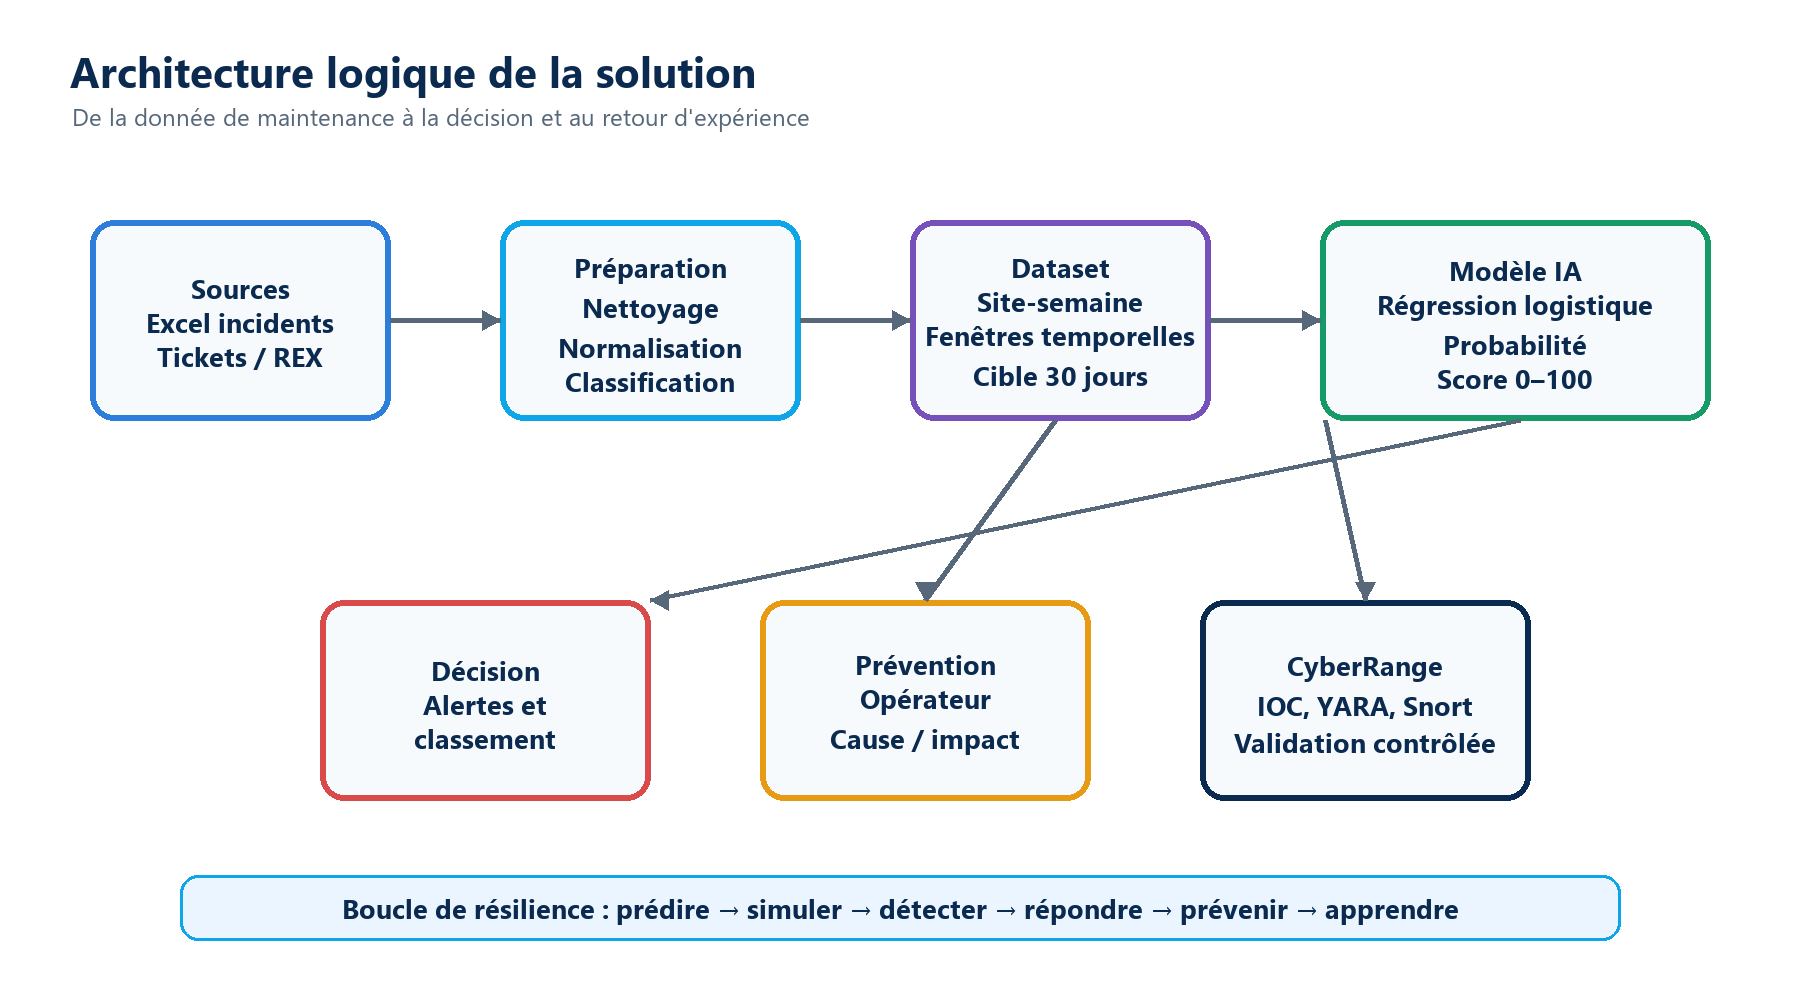
\includegraphics[width=0.95\textwidth,keepaspectratio]{images/diagrams/solution_pipeline.png}
\caption[Chaîne intégrée]{Chaîne intégrée : prédire, simuler, détecter, remédier et capitaliser.}
\end{figure}

\section{Méthode de développement}

Le développement suit une démarche itérative inspirée de Scrum. Le binôme découpe le projet en incréments : compréhension du besoin, préparation des données, construction du modèle, réalisation des interfaces, intégration du facteur humain, validation CyberRange et rédaction. Chaque incrément est vérifié à partir de critères observables : cohérence des données, lisibilité du score, fonctionnement des parcours, isolement du laboratoire et traçabilité des résultats.

À chaque itération, nous avons cherché à produire un résultat démontrable plutôt qu’une fonctionnalité isolée. La préparation des données devait alimenter une première mesure ; le modèle devait être visible dans une interface ; la checklist devait déclencher un état de conformité ; la simulation devait fournir des preuves et une recommandation défensive. Cette logique permet de vérifier progressivement que les composants contribuent bien au même objectif de prévention.

\section{Planification prévisionnelle}

\begin{table}[H]
\centering
\small
\caption{Planification synthétique du projet.}
\begin{tabularx}{\textwidth}{B{4.0cm} P{5.0cm} X}
\toprule
Itération & Travaux principaux & Livrable\\
\midrule
S1 & Cadrage ONDA, collecte des attentes et inventaire des données & Périmètre et objectifs\\
S2 & Nettoyage, exploration et définition des indicateurs & Jeu de données documenté\\
S3 & Entraînement et évaluation du modèle & Score et métriques\\
S4 & Portail exécutif et module d’alertes & Interfaces de pilotage\\
S5 & Facteur humain, checklist et REX & Module opérationnel\\
S6 & Prévention WAN, opérateurs et prévisions & Plan d’action\\
S7 & CyberRange isolé et collecte des preuves & Scénario de validation\\
S8 & Intégration, tests et rédaction & Version finale du rapport\\
\bottomrule
\end{tabularx}
\end{table}

\section{Conclusion}

Le contexte ONDA justifie une approche qui dépasse le simple affichage de tickets. La solution retenue transforme l’historique de maintenance en priorités prédictives et ajoute un laboratoire CyberRange pour relier disponibilité, sécurité et REX. Le chapitre suivant précise les besoins fonctionnels, les contraintes et les acteurs de cette solution.

Le cadre de projet est donc défini par un équilibre entre ambition et maîtrise du périmètre. Les fonctionnalités livrées sont suffisamment larges pour couvrir la décision, la prévention et la validation, tout en restant compatibles avec les données disponibles et avec un environnement de démonstration. Cette base permet maintenant de formaliser les attentes des utilisateurs et les conditions de qualité à respecter.

\ChapterDivider{Spécification des besoins}

\section{Introduction}

La spécification traduit le problème métier en services attendus par les utilisateurs. Elle distingue les fonctions visibles dans la plateforme, les contraintes de qualité et de sécurité, puis formalise les interactions entre acteurs et système.

La spécification prend en compte des profils qui ne consultent pas le système avec le même niveau de détail. Un directeur recherche une synthèse et des priorités, un ingénieur veut comprendre les facteurs du score, un technicien a besoin de contrôles pratiques et un analyste sécurité examine des preuves. La solution doit donc offrir plusieurs niveaux de lecture sans perdre la cohérence des informations affichées.

\section{Acteurs du système}

\begin{table}[H]
\centering
\small
\caption{Acteurs et responsabilités.}
\begin{tabularx}{\textwidth}{B{4.0cm} X}
\toprule
Acteur & Responsabilité\\
\midrule
Administrateur DSI & Accéder à la vision globale, gérer les droits et contrôler les indicateurs.\\
Ingénieur réseau & Examiner les alertes, les historiques, les causes et les actions de mitigation.\\
Responsable maintenance & Prioriser les interventions, suivre les opérateurs et vérifier la prévention.\\
Analyste sécurité & Observer les preuves du CyberRange, vérifier les indicateurs et proposer une remédiation.\\
Technicien & Exécuter les checklists, documenter l’intervention et contribuer au REX.\\
Opérateur télécom & Recevoir les escalades et traiter les incidents de liaison.\\
\bottomrule
\end{tabularx}
\end{table}

\section{Besoins fonctionnels}

Les besoins fonctionnels sont organisés autour d’un cycle de prévention. Le système doit d’abord observer les historiques, ensuite produire une estimation, puis permettre la vérification humaine et le suivi de l’action. La simulation de sécurité suit le même principe : préparer un scénario, observer les événements, vérifier les détections et consigner les mesures correctives. Chaque fonction est associée à un résultat visible pour éviter que la prédiction ou la preuve ne reste sans suite opérationnelle.

\begin{itemize}
  \item BF1 — Afficher une vue exécutive de l’état du réseau et de la distribution des niveaux de risque.
  \item BF2 — Calculer et classer un score de risque compris entre 0 et 100 pour chaque site.
  \item BF3 — Filtrer les alertes par niveau, rechercher un site et ouvrir sa fiche détaillée.
  \item BF4 — Consulter l’historique, les catégories d’incidents, la durée d’indisponibilité et la date du dernier incident.
  \item BF5 — Diagnostiquer le modèle à l’aide de métriques, d’une matrice de confusion et d’une courbe de comparaison.
  \item BF6 — Analyser les causes, les opérateurs et les saisonnalités pour générer des recommandations à 30 jours.
  \item BF7 — Contrôler une intervention par checklist, déclarer une erreur et enregistrer un REX.
  \item BF8 — Reproduire un scénario de sécurité en laboratoire isolé, collecter les preuves et relier la remédiation au REX.
\end{itemize}

\section{Besoins non fonctionnels}

Les exigences non fonctionnelles sont importantes car la plateforme traite des informations liées à la disponibilité d’un service critique. La transparence du modèle, la protection des données, la continuité d’accès et l’isolement de la simulation sont aussi importants que la présence d’un graphique. Les choix de conception doivent donc favoriser la lisibilité, la vérifiabilité et la possibilité de revenir sur la décision prise.

\begin{table}[H]
\centering
\small
\caption{Exigences non fonctionnelles.}
\begin{tabularx}{\textwidth}{B{4.0cm} X}
\toprule
Qualité & Exigence\\
\midrule
Sécurité & Le CyberRange doit être isolé du réseau de production et les données sensibles doivent être limitées.\\
Traçabilité & Les recommandations, actions et REX doivent être datés et associés à un site ou à un scénario.\\
Lisibilité & Les niveaux de risque doivent être visibles au premier regard et expliqués par des indicateurs.\\
Reproductibilité & Les versions des données, du modèle et du scénario de test doivent être identifiables.\\
Performance & Les tableaux et graphiques doivent rester consultables avec un volume de tickets historique.\\
Maintenabilité & Les modules doivent être séparés afin de permettre l’évolution du score et des règles.\\
Portabilité & La solution doit pouvoir être exécutée dans un environnement Python documenté.\\
Responsabilité & Les alertes sont une aide à la décision et doivent être validées par un responsable humain.\\
\bottomrule
\end{tabularx}
\end{table}

\section{Cas d’utilisation}

Le diagramme global regroupe les parcours principaux autour de quatre familles : piloter le réseau, analyser le risque, prévenir l’incident et capitaliser l’expérience. Le CyberRange n’est pas un module autonome destiné à lancer des actions sur une cible quelconque ; il est un cas d’utilisation de validation défensive, réalisé dans un périmètre explicitement autorisé.

\begin{figure}[H]
\centering
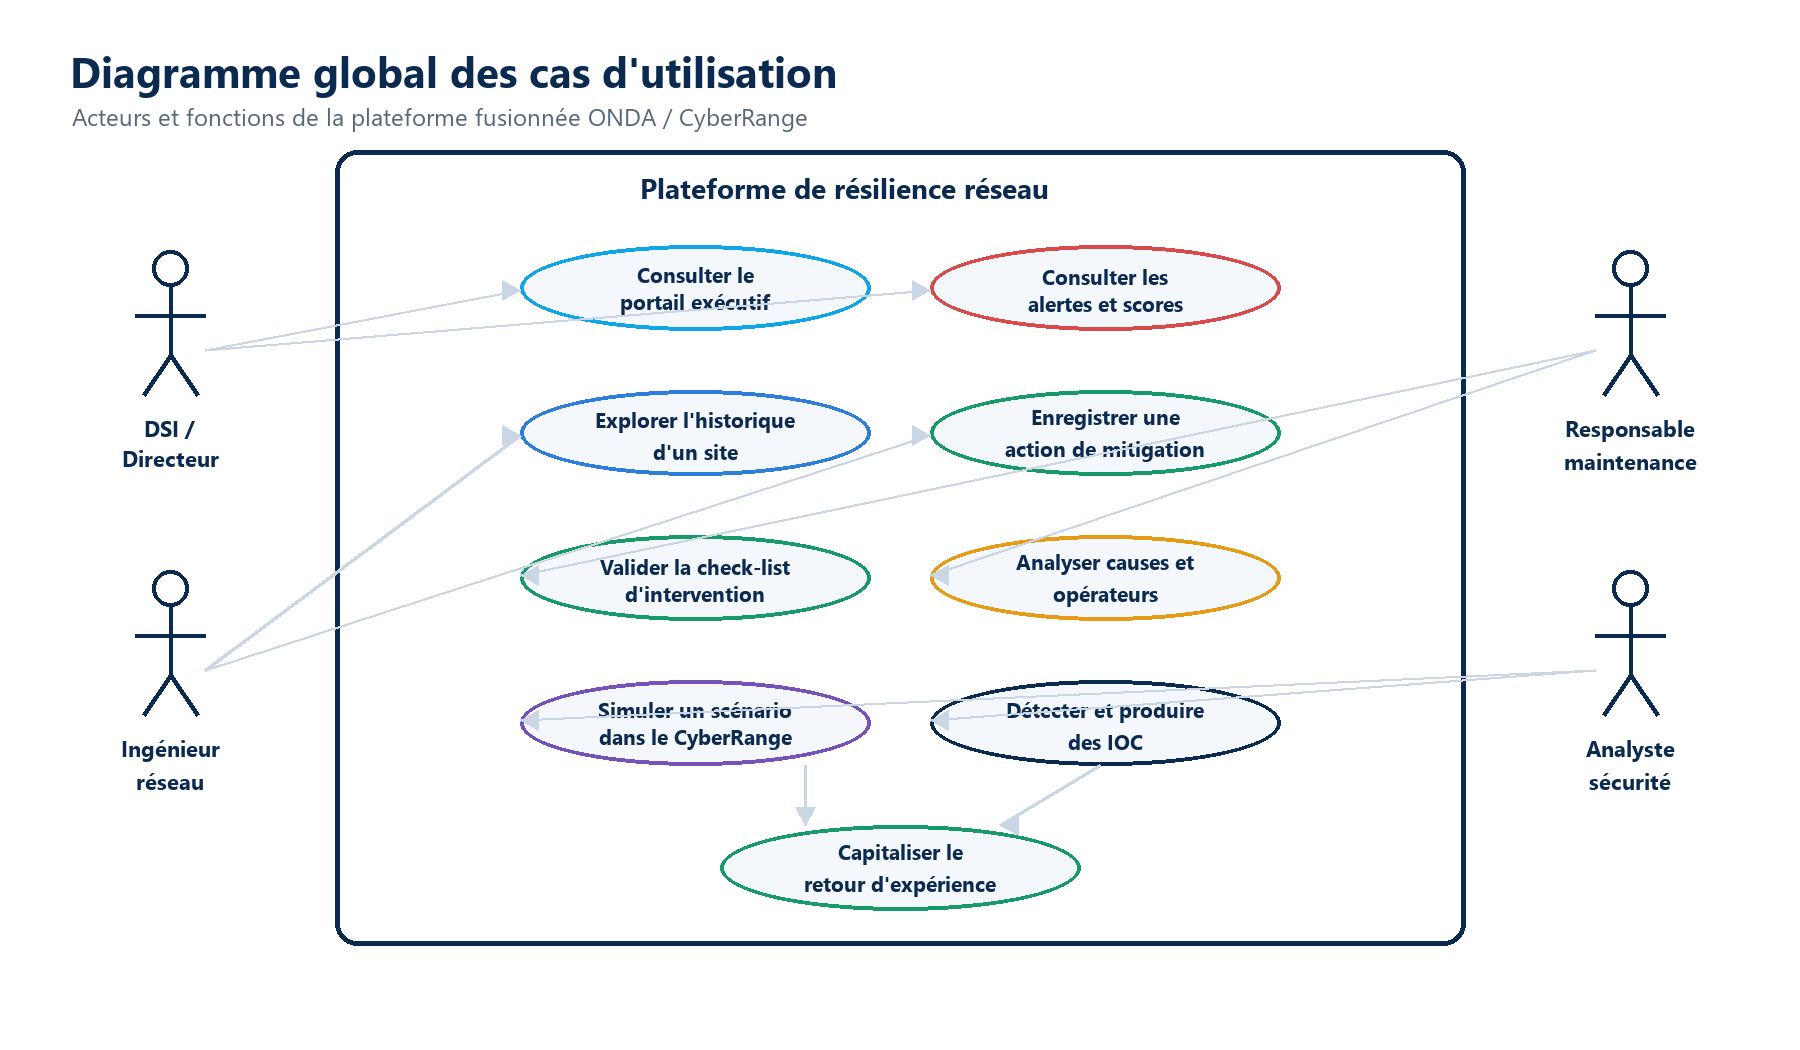
\includegraphics[width=0.96\textwidth,keepaspectratio]{images/diagrams/usecase_global.png}
\caption[Diagramme global des cas d’utilisation.]{Diagramme global des cas d’utilisation.}
\end{figure}

\section{Description de cas d’utilisation représentatifs}

\subsection{Consulter les alertes de risque}

L’acteur ouvre le module de risque et sélectionne éventuellement un niveau ou un site. Le système charge le classement, affiche les éléments les plus critiques et permet d’ouvrir une fiche détaillée. Le résultat attendu est une liste priorisée, accompagnée des facteurs qui expliquent le score.

Le prérequis est la disponibilité d’un jeu de données préparé et d’un modèle identifié. Le scénario nominal se termine lorsque l’utilisateur dispose d’un site prioritaire et de ses indicateurs de contexte. En cas de données incomplètes, le système doit signaler la limite plutôt que présenter un score comme une certitude ; cette règle protège la qualité de la décision.

\subsection{Générer un plan de prévention}

Le responsable maintenance consulte les causes et les opérateurs, puis ouvre l’onglet des prévisions. Le système agrège l’historique et produit des recommandations telles que la vérification de l’alimentation secourue, la planification d’une mission technique ou l’escalade vers un opérateur.

La recommandation est ensuite transformée en action suivie : responsable, priorité, échéance et commentaire. Le système doit permettre de distinguer une action proposée d’une action confirmée, puis d’une action réalisée. Cette distinction est nécessaire pour évaluer plus tard si une prévention a effectivement réduit le risque ou si elle doit être adaptée.

\subsection{Valider une intervention}

Avant une modification, le technicien sélectionne le type d’intervention et coche les prérequis : sauvegarde de configuration, contrôle d’intégrité, fenêtre horaire, notification, rollback et vérification post-opération. Le système calcule un taux de conformité et signale un risque humain si des contrôles impératifs manquent.

Le parcours prévoit également un arrêt préventif. Si un contrôle critique n’est pas validé, l’intervention ne doit pas être considérée comme conforme, même si les autres cases sont cochées. Après l’opération, le technicien peut compléter le commentaire, joindre une preuve et signaler une difficulté rencontrée. Ces informations enrichissent le REX et contribuent à réduire la répétition des erreurs.

\subsection{Examiner une simulation de sécurité}

L’analyste sécurité exécute un scénario autorisé dans l’environnement Host-Only, observe les preuves réseau et système, puis consigne les indicateurs, les règles de détection et les mesures de remédiation. Le scénario est considéré comme un élément de validation et non comme un accès à une infrastructure réelle.

Le résultat attendu est un dossier de validation comprenant le périmètre, les hôtes de test, la chronologie, les observations, les alertes obtenues et les mesures recommandées. Une simulation incomplète reste utile si elle permet d’identifier un manque de visibilité ou une règle à améliorer. La priorité est donnée à la compréhension et à la défense, sans publier de procédure offensive applicable à un système tiers.

\section{Conclusion}

Les besoins montrent que la plateforme doit fournir à la fois une vue synthétique, des analyses explicables et des actions contrôlées. La spécification couvre la continuité WAN, le facteur humain et la sécurité de laboratoire dans un même parcours. La conception de ces flux et de leurs données est présentée au chapitre suivant.

Cette spécification fournit un critère de vérification pour la suite du projet : chaque interface, chaque indicateur et chaque capture doit pouvoir être rattaché à un besoin identifié. Elle évite également de confondre l’objectif de prédiction avec celui de simulation. L’un aide à prioriser la maintenance ; l’autre vérifie la préparation à la détection et à la remédiation dans un cadre isolé.

\ChapterDivider{Conception du système}

\section{Introduction}

La conception décrit les échanges entre les composants, la structure des données et l’architecture de déploiement. Elle tient compte du caractère hybride du projet : l’analyse prédictive s’appuie sur des historiques de maintenance, tandis que le CyberRange est un environnement de test isolé qui fournit des preuves complémentaires.

Un principe de conception guide l’ensemble du système : conserver la traçabilité entre une donnée source et la décision produite. Un score doit pouvoir être expliqué par une période, un site et des indicateurs ; une recommandation doit être reliée à une cause ou à une tendance ; une preuve CyberRange doit être rattachée à une étape du scénario. Cette traçabilité facilite la validation par les utilisateurs et la rédaction du REX.

\section{Architecture fonctionnelle}

L’architecture fonctionnelle suit une chaîne de traitement en cinq niveaux. Les données sont d’abord préparées, puis transformées en variables temporelles. Le modèle produit une probabilité et un score de risque. Les modules d’interface expliquent les résultats et génèrent une action. Enfin, l’exécution et les preuves alimentent le retour d’expérience.

La chaîne sépare les opérations de calcul des opérations de présentation. Les agrégations temporelles sont réalisées avant l’affichage afin que les différentes vues utilisent les mêmes valeurs. Le portail ne recalcule pas une interprétation différente pour chaque écran : il restitue un référentiel commun, ce qui réduit les incohérences entre le tableau de bord, la fiche d’un site et le plan de prévention.

\begin{figure}[H]
\centering
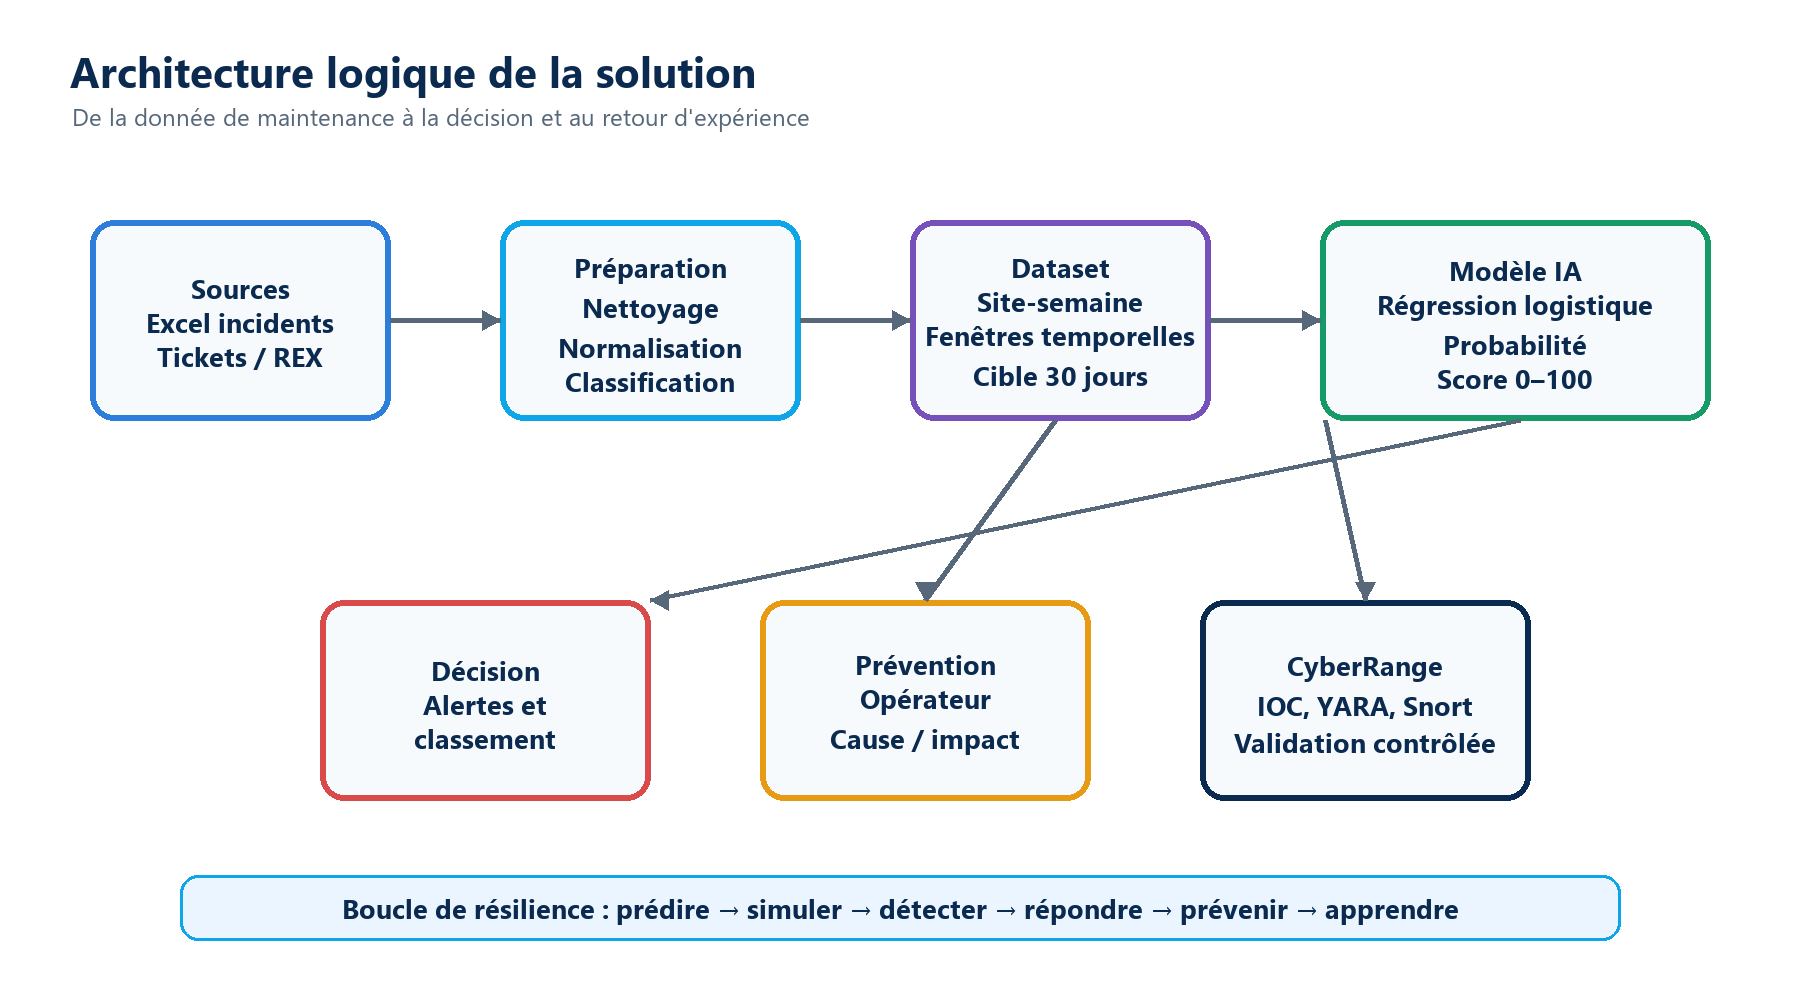
\includegraphics[width=0.95\textwidth,keepaspectratio]{images/diagrams/solution_pipeline.png}
\caption[Architecture fonctionnelle de la solution intégrée.]{Architecture fonctionnelle de la solution intégrée.}
\end{figure}

\section{Modélisation dynamique}

\subsection{Séquence d’une alerte prédictive}

La séquence commence par l’import ou la mise à jour des tickets. Le service de préparation calcule les fenêtres temporelles, puis le modèle évalue la probabilité d’incident. Le portail classe les sites et le responsable valide l’action. Une intervention peut déclencher la checklist ; une simulation peut produire des preuves de détection ; dans les deux cas, les résultats sont capitalisés dans le REX.

Le flux prévoit un contrôle avant la diffusion de l’alerte. Les dates doivent être cohérentes, le site doit appartenir au référentiel et les valeurs nécessaires au calcul doivent être disponibles. Si une anomalie est détectée, elle doit être signalée à l’utilisateur ou exclue du calcul selon une règle documentée. Cette étape évite de donner une apparence de précision à une prédiction fondée sur une donnée incorrecte.

\begin{figure}[H]
\centering
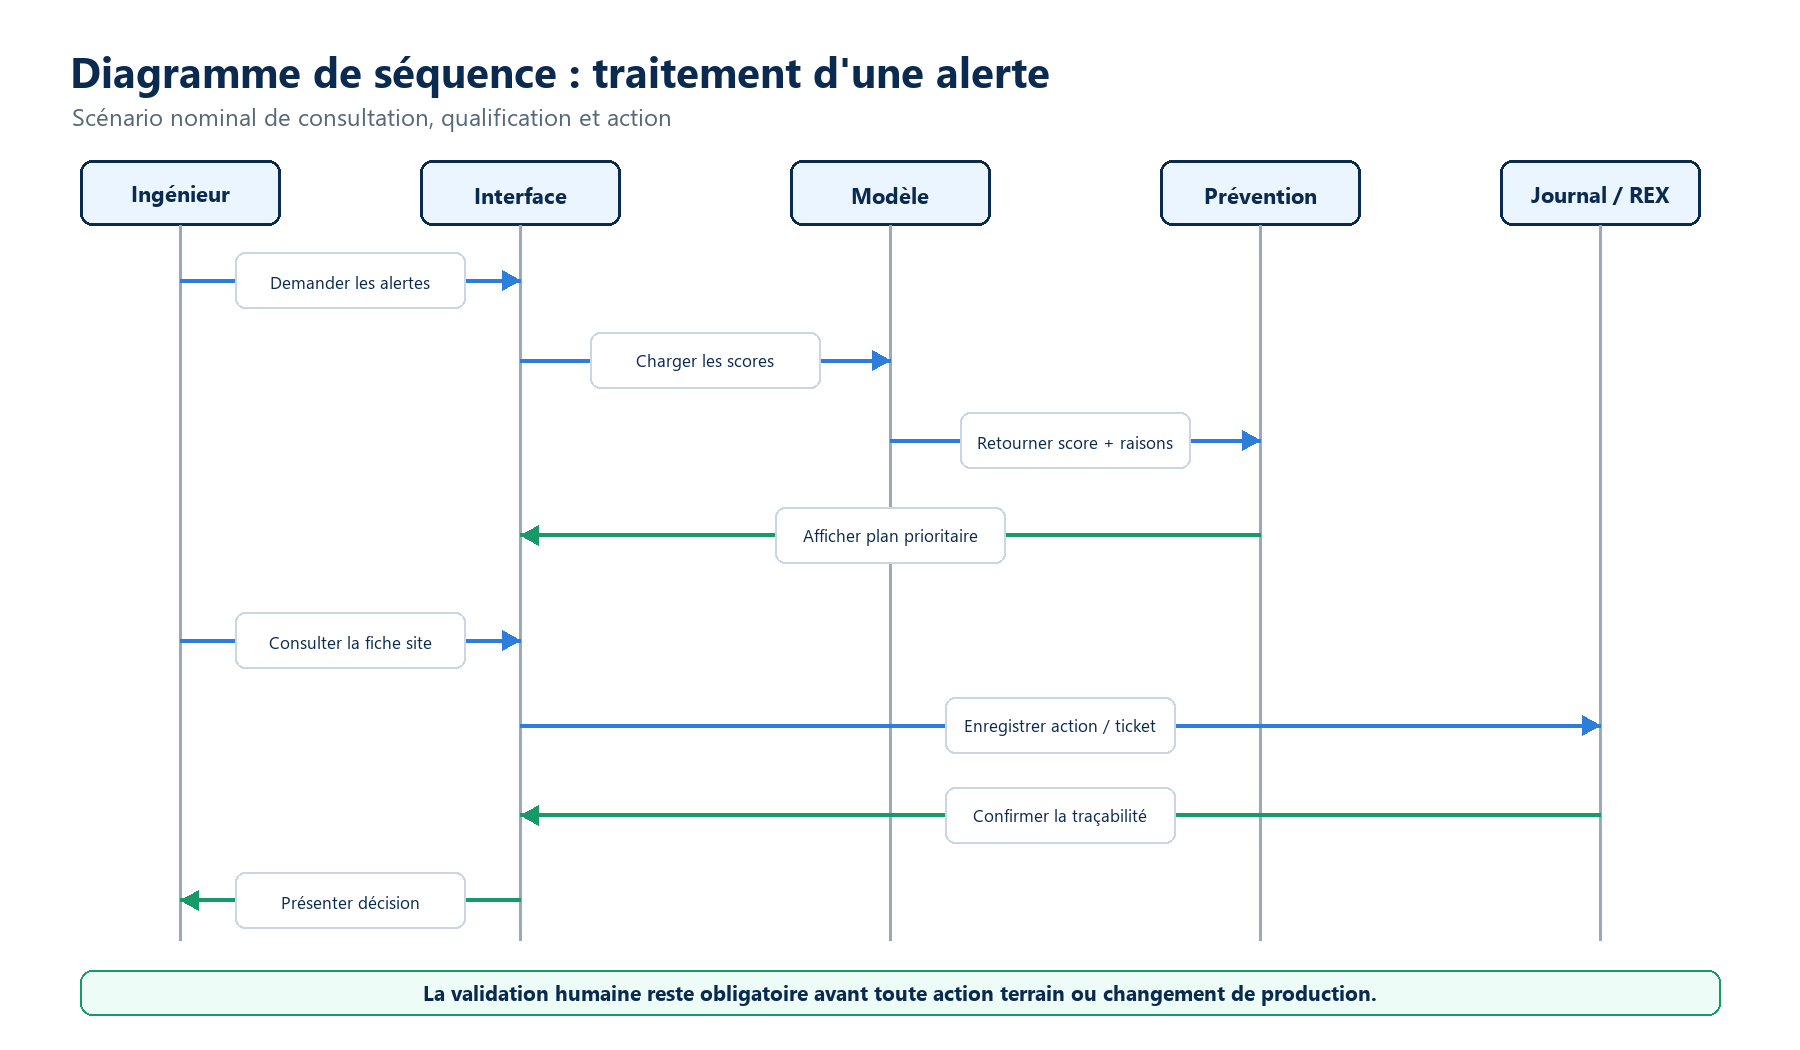
\includegraphics[width=0.95\textwidth,keepaspectratio]{images/diagrams/sequence_alert.png}
\caption[Séquence de production d’une alerte et de capitalisation.]{Séquence de production d’une alerte et de capitalisation.}
\end{figure}

\subsection{Activité globale}

\begin{itemize}
  \item Importer les tickets et contrôler la qualité des dates, sites, catégories et durées.
  \item Construire les variables récentes et historiques sans utiliser d’informations futures.
  \item Produire le score et affecter un niveau de risque selon les seuils retenus.
  \item Afficher l’alerte, vérifier l’impact et sélectionner une action de prévention.
  \item Contrôler l’intervention ou analyser les preuves CyberRange.
  \item Enregistrer la décision, les résultats et le REX.
\end{itemize}

\section{Modélisation statique et modèle de données}

Le modèle de données relie les sites, les incidents, les prédictions, les actions de maintenance et les retours d’expérience. L’entité ScenarioCyberRange conserve la référence d’un scénario isolé et ses preuves, mais ne mélange pas les données de simulation avec les tickets de production. Cette séparation limite les ambiguïtés d’interprétation.

Les relations sont pensées pour conserver l’historique. Une nouvelle prédiction ne doit pas écraser la précédente, car l’évolution du score peut être utile pour mesurer l’effet d’une action. De même, une action de maintenance peut être associée à plusieurs observations et un REX peut référencer un incident, une intervention ou une simulation. Cette approche permet d’étudier non seulement le risque, mais aussi la réponse apportée.

\begin{figure}[H]
\centering
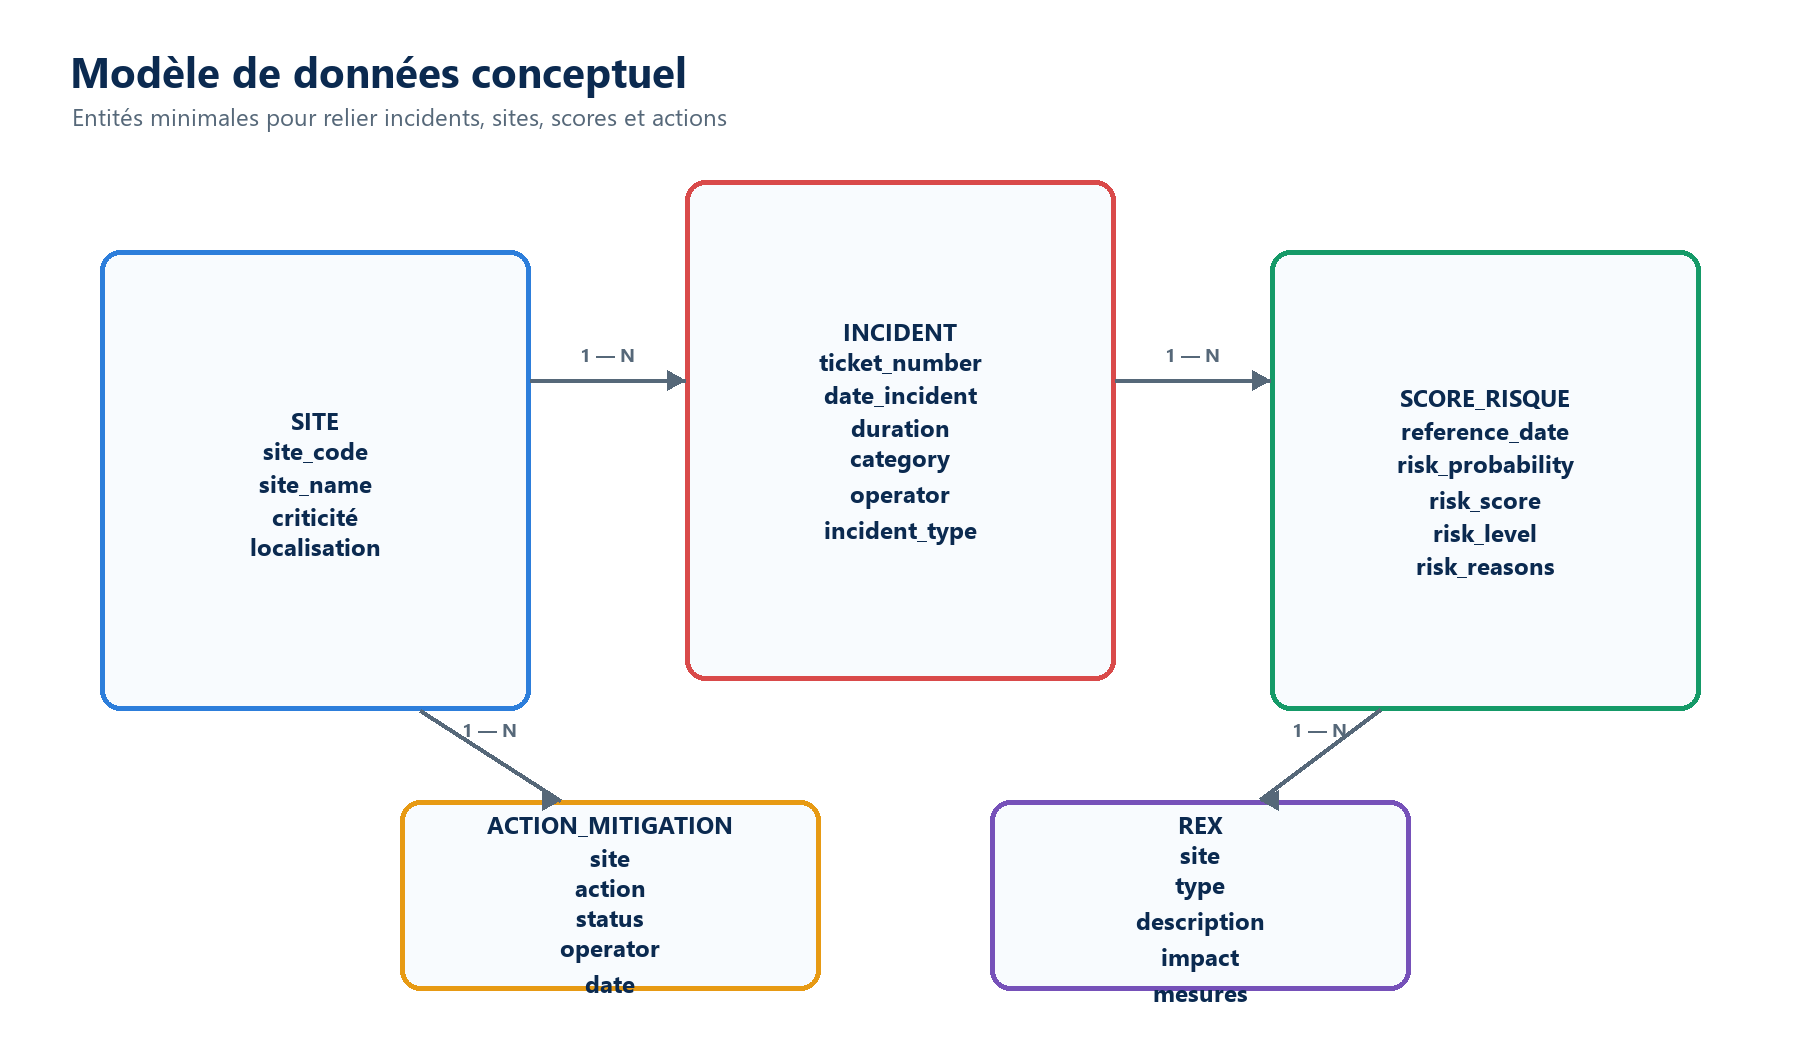
\includegraphics[width=0.95\textwidth,keepaspectratio]{images/diagrams/data_model.png}
\caption[Modèle logique simplifié des données.]{Modèle logique simplifié des données.}
\end{figure}

\begin{table}[H]
\centering
\small
\caption{Dictionnaire synthétique des données.}
\begin{tabularx}{\textwidth}{B{4.0cm} P{5.0cm} X}
\toprule
Entité & Attributs principaux & Rôle\\
\midrule
Site & id\_site, code, nom, région & Référentiel des 27 sites suivis.\\
Incident & id, site, date, catégorie, opérateur, durée & Historique des événements WAN.\\
Prediction & site, date, probabilité, score, niveau & Résultat calculé par le modèle.\\
ActionMaintenance & site, type, statut, date, commentaire & Suivi des mesures préventives.\\
Checklist & intervention, prérequis, conformité & Contrôle des étapes avant production.\\
REX & auteur, contexte, cause, action, date & Capitalisation des enseignements.\\
ScenarioCyberRange & id, hôtes, scénario, preuves, remédiation & Validation sécurité isolée.\\
\bottomrule
\end{tabularx}
\end{table}

\section{Architecture logicielle}

La plateforme est organisée en modules Python correspondant aux responsabilités fonctionnelles. home.py porte la vue exécutive ; app.py regroupe l’analyse de risque et le diagnostic du modèle ; human\_factor.py gère checklist, erreurs et REX ; prevention.py regroupe l’analyse des causes, opérateurs et prévisions. Les composants de visualisation et de préparation des données sont appelés par ces modules, ce qui facilite les évolutions.

Cette organisation rend les tests plus simples. Les fonctions de préparation peuvent être vérifiées indépendamment du rendu graphique, les règles de checklist peuvent être testées avec plusieurs états de conformité et les indicateurs de prévention peuvent être comparés aux agrégations historiques. L’interface devient ainsi une couche de restitution, tandis que les règles métier restent identifiables et modifiables.

\section{Architecture matérielle et déploiement}

Le portail est consulté depuis un poste DSI via un navigateur. La couche applicative exécute les calculs et restitue les tableaux de bord. Les données historiques sont stockées dans un espace contrôlé. Le CyberRange est déployé séparément dans VirtualBox avec un réseau Host-Only, de sorte que les machines de test communiquent entre elles sans accès à Internet ni au réseau de production.

Le déploiement doit aussi prendre en compte la gestion des versions et des sauvegardes. Le modèle, les fichiers de données, les règles de détection et les captures doivent être conservés avec un identifiant ou une date de référence. En cas de réentraînement, l’équipe doit pouvoir comparer les métriques et comprendre pourquoi le classement des sites a changé. Cette discipline est indispensable avant toute utilisation régulière de l’outil.

\begin{figure}[H]
\centering
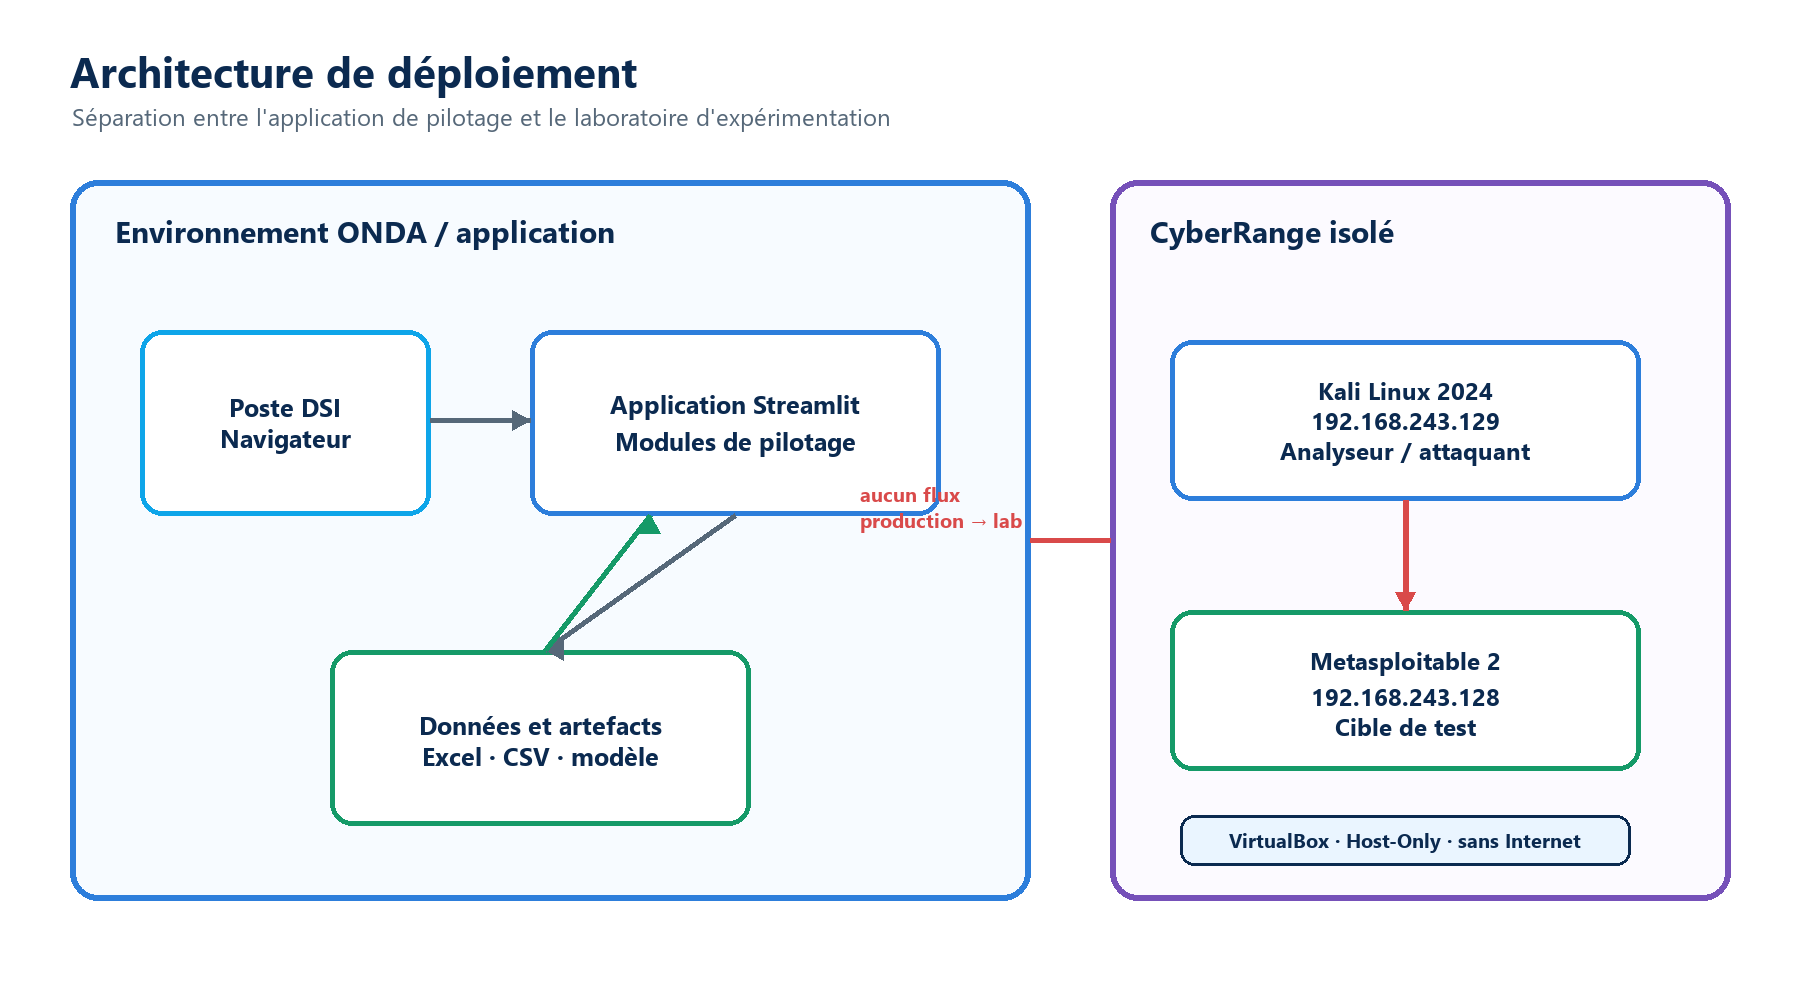
\includegraphics[width=0.95\textwidth,keepaspectratio]{images/diagrams/deployment_architecture.png}
\caption[Architecture de déploiement et périmètre isolé du CyberRange.]{Architecture de déploiement et périmètre isolé du CyberRange.}
\end{figure}

\section{Principes de sécurité de la simulation}

\begin{itemize}
  \item Utiliser uniquement des machines vulnérables prévues pour l’entraînement, notamment Metasploitable 2.
  \item Maintenir le mode Host-Only et vérifier l’absence de route vers Internet avant l’exercice.
  \item Ne pas réutiliser les charges, identifiants ou indicateurs sur une infrastructure réelle.
  \item Conserver les captures comme preuves de laboratoire, avec leur contexte et leur date.
  \item Associer chaque observation à une mesure défensive : détection, durcissement, segmentation ou remédiation.
\end{itemize}

\section{Conclusion}

La conception relie le score de risque aux flux opérationnels et maintient une séparation nette entre la production et la simulation. Les modèles de données, la séquence d’alerte et l’architecture Host-Only fournissent une base cohérente pour la réalisation. Les interfaces et les résultats obtenus sont présentés dans le dernier chapitre.

Les choix de conception donnent donc une place centrale à l’explicabilité et à la sécurité du périmètre. Le système est capable de produire un résultat exploitable, mais il conserve les conditions nécessaires à son interprétation : origine de la donnée, période d’analyse, responsable de la décision et environnement de validation. Cette cohérence constitue le lien entre la conception théorique et les éléments réalisés.

\ChapterDivider{Réalisation du système}

\section{Introduction}

Ce chapitre présente l’environnement de réalisation, les interfaces de la plateforme ONDA, les résultats du modèle et la validation complémentaire menée dans le CyberRange. Les captures sont utilisées comme éléments de preuve visuelle de la solution et du laboratoire de test.

La réalisation est présentée dans l’ordre d’utilisation. Nous commençons par la préparation des données et l’évaluation, puis nous décrivons les écrans qui rendent les résultats accessibles aux différents profils. Nous terminons par le scénario CyberRange, qui montre comment les observations de sécurité peuvent être documentées et réinjectées dans une démarche de prévention.

\section{Environnement matériel et logiciel}

L’environnement de développement a été choisi pour permettre une expérimentation reproductible et une présentation claire des résultats. Les outils de traitement servent à préparer les historiques et à calculer les indicateurs ; les outils de visualisation rendent ces indicateurs accessibles ; VirtualBox fournit un périmètre séparé pour la simulation. Les versions et les paramètres importants doivent être conservés avec le projet afin de faciliter une reprise ultérieure.

\begin{table}[H]
\centering
\small
\caption{Environnement de réalisation.}
\begin{tabularx}{\textwidth}{B{4.0cm} X}
\toprule
Composant & Technologies / configuration\\
\midrule
Développement & Python, notebooks/scripts d’analyse, environnement virtuel documenté.\\
Interface & Application web Python avec tableaux, graphiques, filtres et formulaires.\\
Données & Historique des incidents WAN et variables temporelles par site.\\
Modèle & Régression logistique pour une classification binaire et un score probabiliste.\\
Simulation & VirtualBox, Kali Linux 2024 et Metasploitable 2.\\
Observation & Wireshark, traces réseau, analyse statique et règles de détection.\\
\bottomrule
\end{tabularx}
\end{table}

\section{Préparation des données et modèle}

Le jeu exploité contient 864 incidents historiques répartis sur 27 sites. Les variables décrivent notamment les incidents sur 7, 30, 90 et 180 jours, les durées récentes, la moyenne et le maximum de durée, le nombre d’incidents par cause ou opérateur, ainsi que le nombre de jours depuis le dernier incident. La séparation temporelle évite d’entraîner le modèle sur des informations postérieures à la période évaluée.

La préparation commence par l’harmonisation des dates, des codes de site, des catégories et des durées. Les incidents sont ensuite regroupés selon plusieurs fenêtres afin de représenter à la fois une activité récente et un profil historique. Cette représentation est importante : un site peut avoir peu d’incidents dans la dernière semaine tout en conservant une tendance défavorable sur plusieurs mois. Les agrégations permettent au modèle d’exploiter ces deux dimensions.

La cible correspond à l’existence d’un incident dans la période de prédiction. Les variables utilisées pour une date donnée doivent être calculées à partir des informations disponibles avant cette date. Le découpage temporel est donc préférable à un mélange aléatoire des lignes, car il reproduit davantage le fonctionnement réel : entraîner sur le passé, puis évaluer sur une période future.

\begin{table}[H]
\centering
\small
\caption{Paramètres de l’évaluation temporelle.}
\begin{tabularx}{\textwidth}{B{4.0cm} X}
\toprule
Élément & Valeur\\
\midrule
Fenêtre d’entraînement & 2021-12-06 → 2023-12-25 (2 916 observations)\\
Fenêtre de test & 2024-01-01 → 2024-09-23 (1 053 observations)\\
Modèle & Régression logistique\\
Horizon opérationnel & 30 jours\\
Référence de l’interface & 25 octobre 2024\\
\bottomrule
\end{tabularx}
\end{table}

\section{Résultats du modèle}

Le modèle fournit une bonne capacité de rappel, ce qui est cohérent avec un usage de prévention où manquer un site à risque peut être plus coûteux que déclencher une vérification supplémentaire. Les valeurs observées sont : accuracy 62,39 \%, précision 54,70 \%, rappel 88,44 \%, F1-score 67,59 \%, ROC-AUC 0,777 et PR-AUC 0,705. L’interface d’accueil affiche un indicateur arrondi de 62 \% ; il correspond à l’accuracy du modèle et non à la précision au sens strict.

La précision indique la proportion d’alertes réellement associées à un incident, tandis que le rappel mesure la proportion d’incidents retrouvés par le modèle. Dans une logique de prévention, le rappel élevé est utile pour ne pas laisser de côté les sites qui méritent une vérification. En contrepartie, la précision montre qu’une partie des alertes devra être examinée par un professionnel avant de déclencher une intervention.

\begin{table}[H]
\centering
\small
\caption{Matrice de confusion du modèle.}
\begin{tabularx}{\textwidth}{B{4.0cm} P{5.0cm} X}
\toprule
Réalité / prédiction & Sans incident & Incident\\
\midrule
Sans incident & 244 & 342\\
Incident & 54 & 413\\
\bottomrule
\end{tabularx}
\end{table}

Les scores sont une aide à la décision. Ils ne remplacent pas l’expertise de l’équipe réseau, notamment lorsque les données sont incomplètes, que le contexte opérationnel change ou qu’une intervention récente n’est pas encore reflétée dans l’historique.

La matrice de confusion confirme également ce compromis : 413 incidents sont correctement identifiés, tandis que 54 incidents sont classés comme sans incident. Les 342 faux positifs ne doivent pas être interprétés uniquement comme un défaut ; ils représentent des situations où une vérification est proposée sans qu’un incident soit ensuite constaté. Le suivi de ces cas est important pour ajuster les seuils, améliorer les variables et éviter une surcharge des équipes.

\section{Portail exécutif}

\begin{figure}[H]
\centering

\includegraphics[width=0.95\textwidth,keepaspectratio]{images/onda/onda_login.png}
\caption[Écran d’accès réservé au personnel ONDA autorisé.]{Écran d’accès réservé au personnel ONDA autorisé.}
\end{figure}

\begin{figure}[H]
\centering
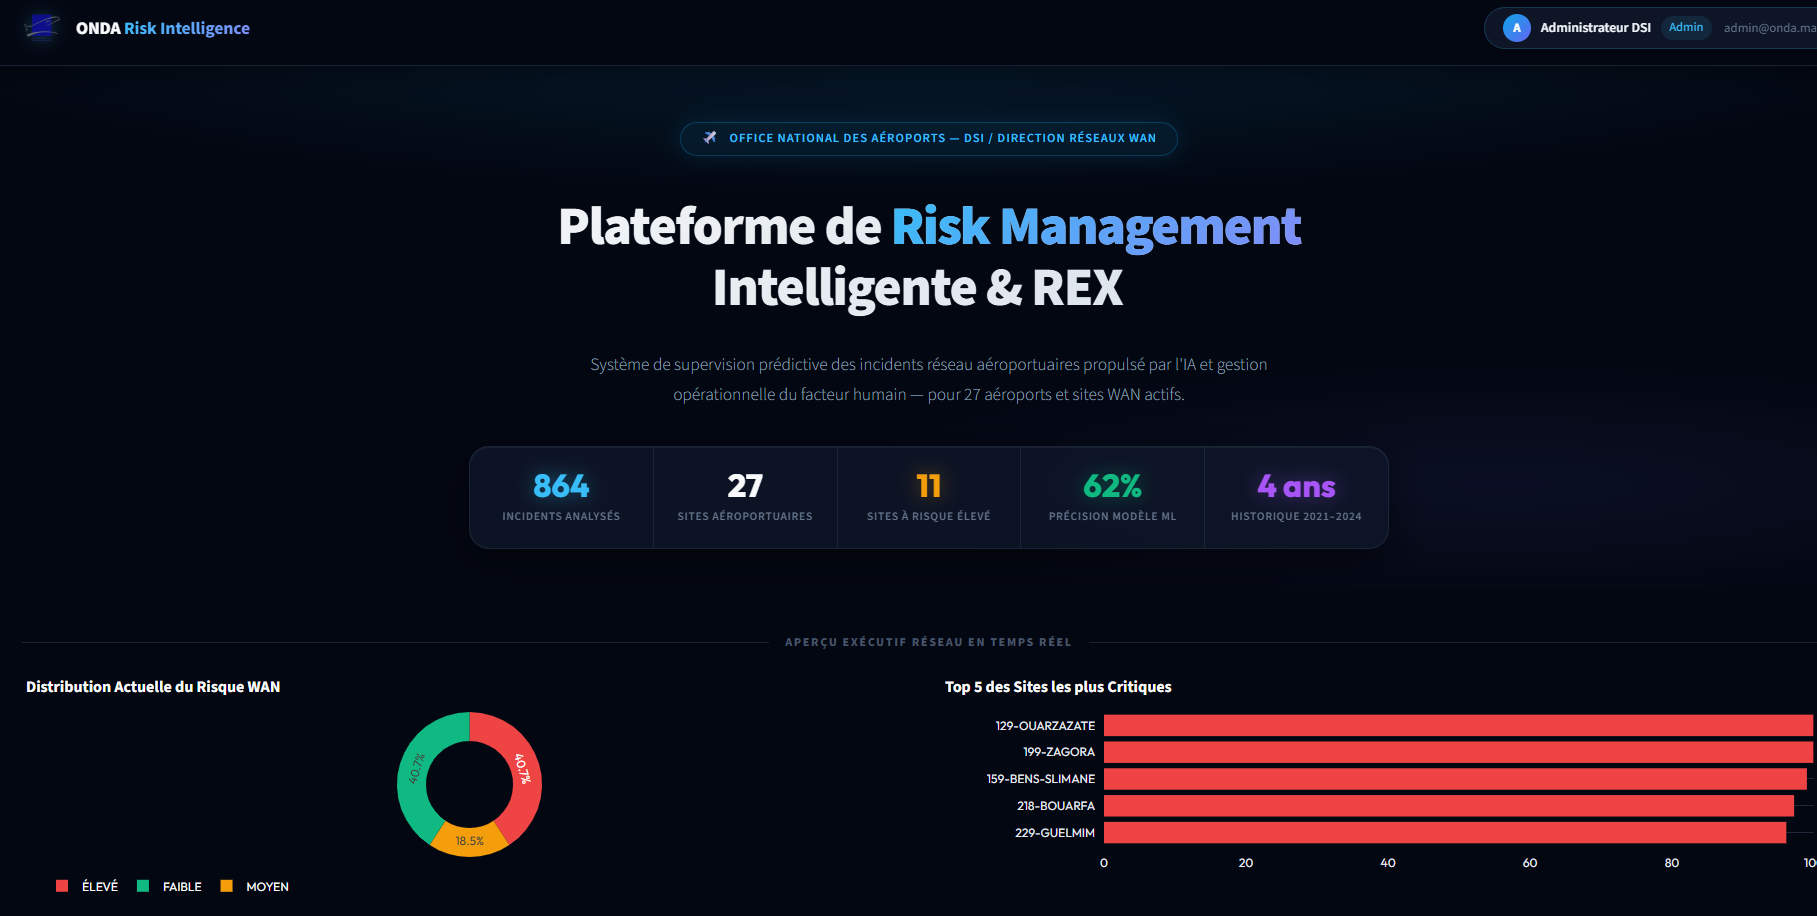
\includegraphics[width=0.95\textwidth,keepaspectratio]{images/onda/onda_home.png}
\caption[Portail exécutif ONDA Risk Intelligence.]{Portail exécutif ONDA Risk Intelligence.}
\end{figure}

\begin{figure}[H]
\centering
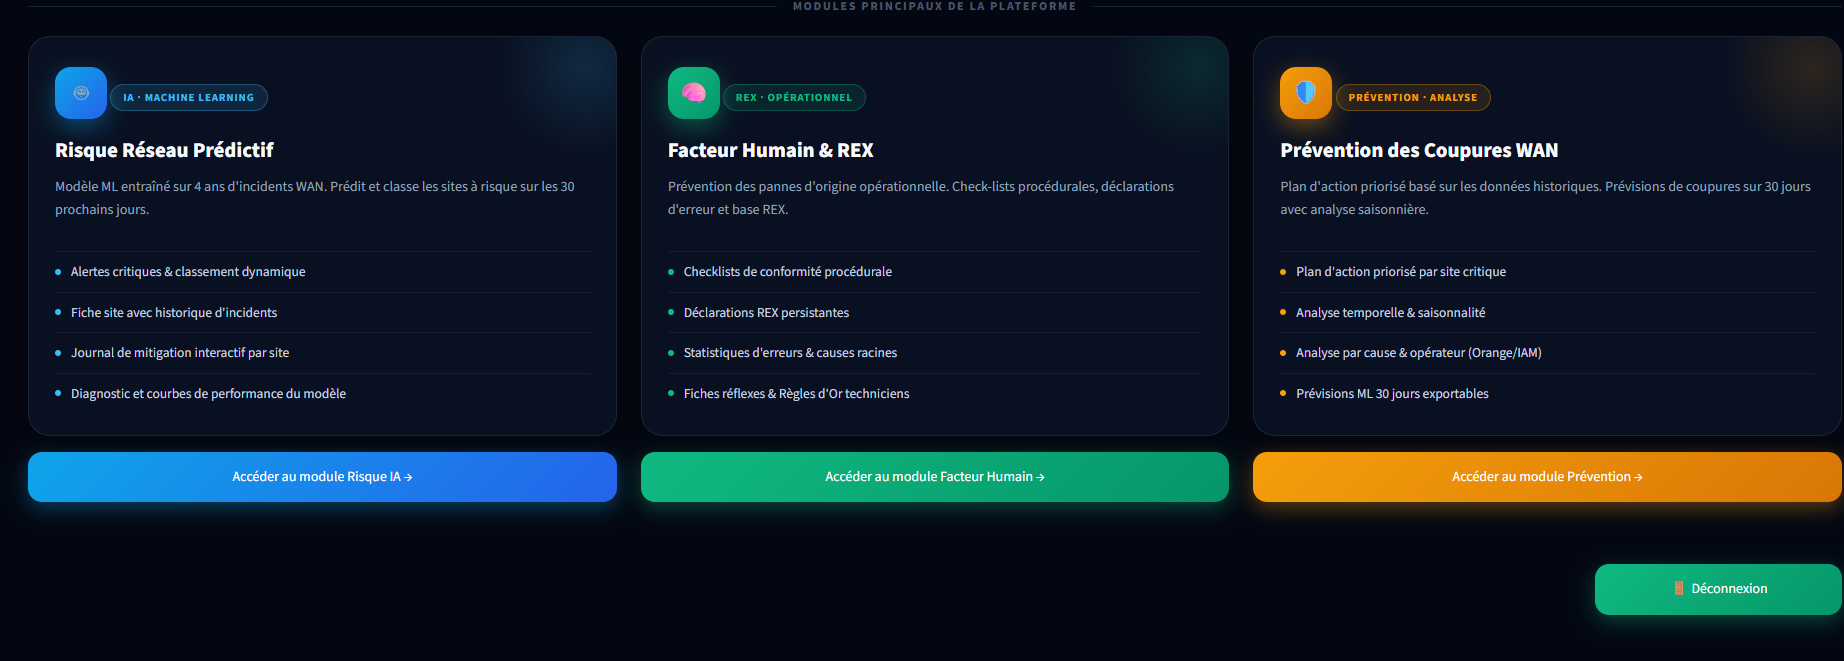
\includegraphics[width=0.95\textwidth,keepaspectratio]{images/onda/onda_modules.png}
\caption[Accès aux trois modules principaux de la plateforme.]{Accès aux trois modules principaux de la plateforme.}
\end{figure}

Le portail exécutif présente les indicateurs de synthèse : incidents analysés, sites suivis, sites à risque élevé, indicateur de performance du modèle et période historique. La distribution des niveaux et le top des sites critiques permettent à un décideur d’identifier rapidement les priorités.

La page d’accueil joue également un rôle de communication. Elle transforme des résultats techniques en une lecture directement compréhensible : le nombre de sites suivis, la proportion de niveaux de risque et le classement des cinq sites prioritaires. Les couleurs servent à distinguer les catégories, mais le texte et les chiffres restent nécessaires pour éviter qu’une couleur seule ne soit prise comme une conclusion.

\section{Module de risque et exploration des sites}

\begin{figure}[H]
\centering
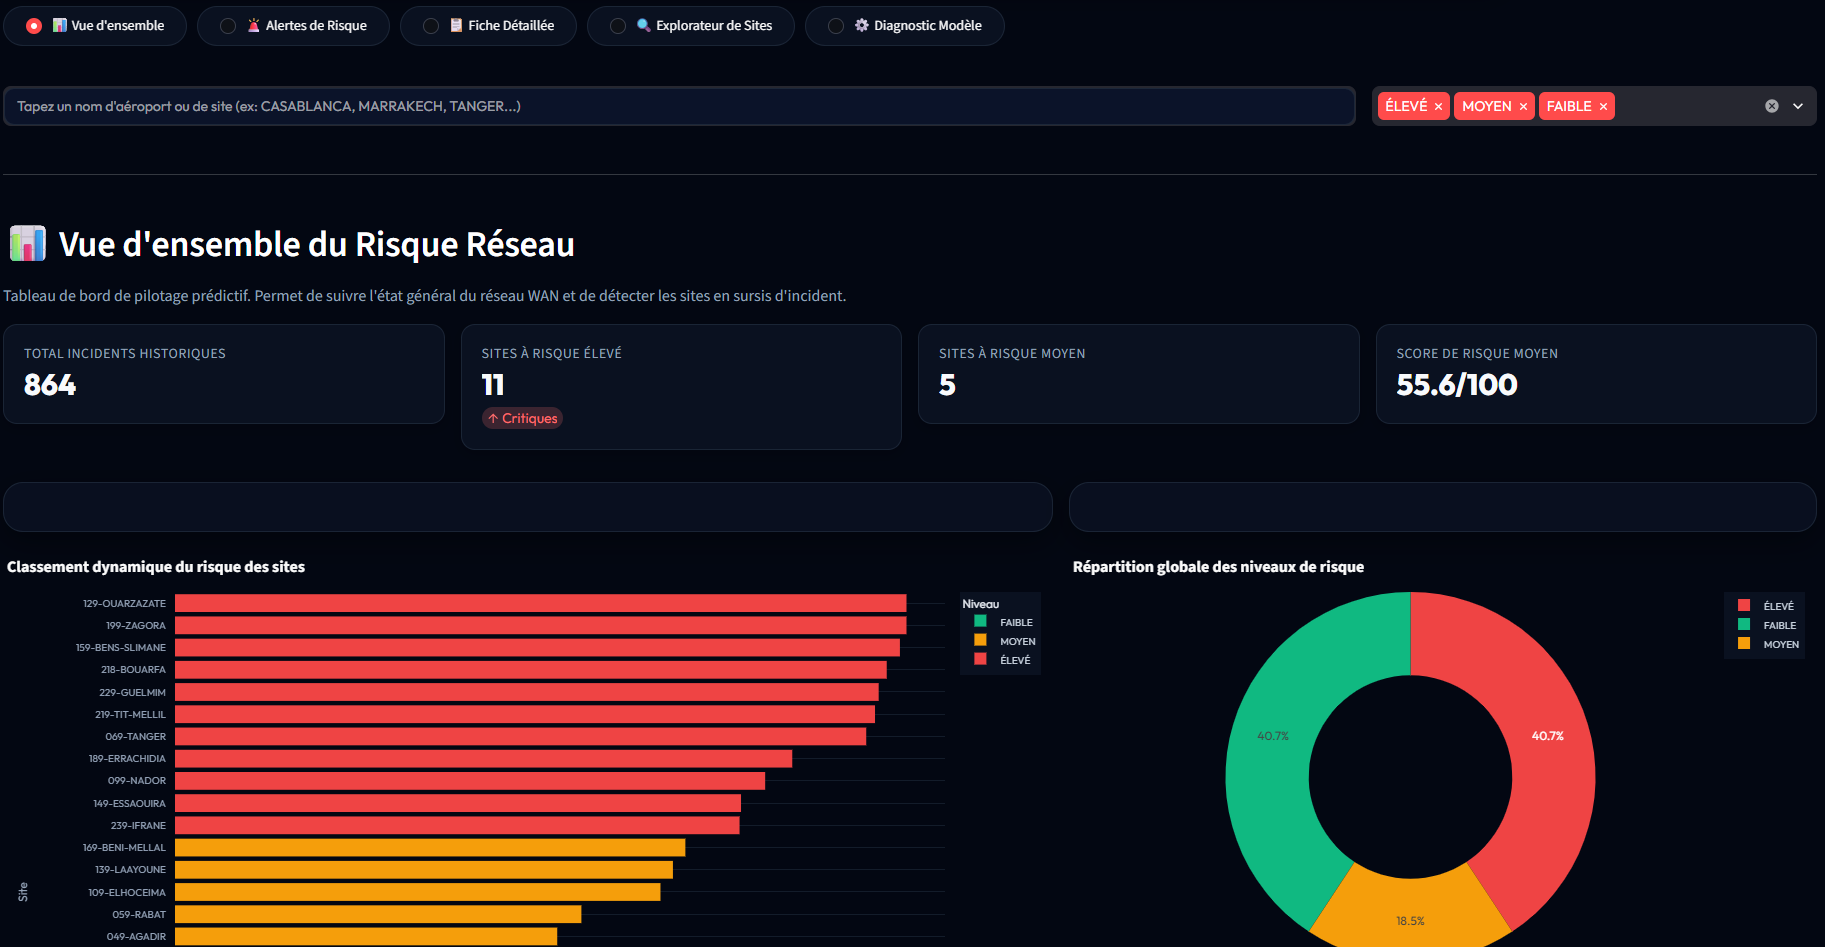
\includegraphics[width=0.95\textwidth,keepaspectratio]{images/onda/onda_overview.png}
\caption[Vue d’ensemble du risque réseau et classement dynamique des sites.]{Vue d’ensemble du risque réseau et classement dynamique des sites.}
\end{figure}

\begin{figure}[H]
\centering
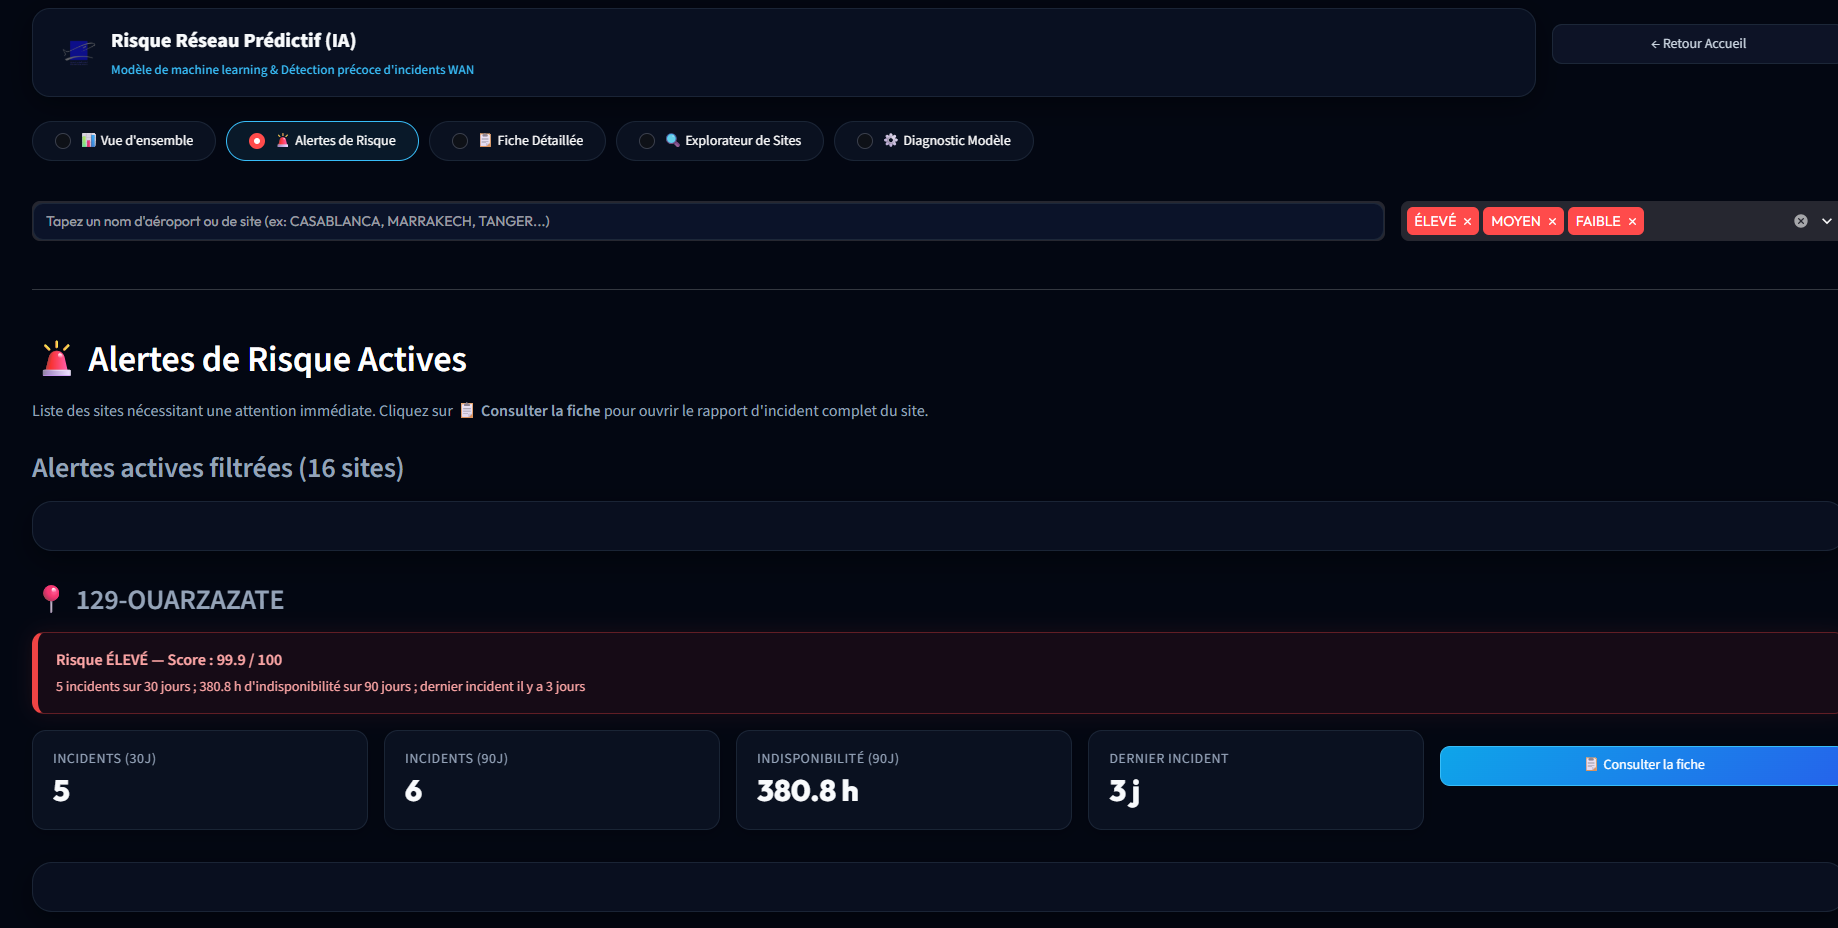
\includegraphics[width=0.95\textwidth,keepaspectratio]{images/onda/onda_alerts.png}
\caption[Liste des alertes de risque actives.]{Liste des alertes de risque actives.}
\end{figure}

\begin{figure}[H]
\centering
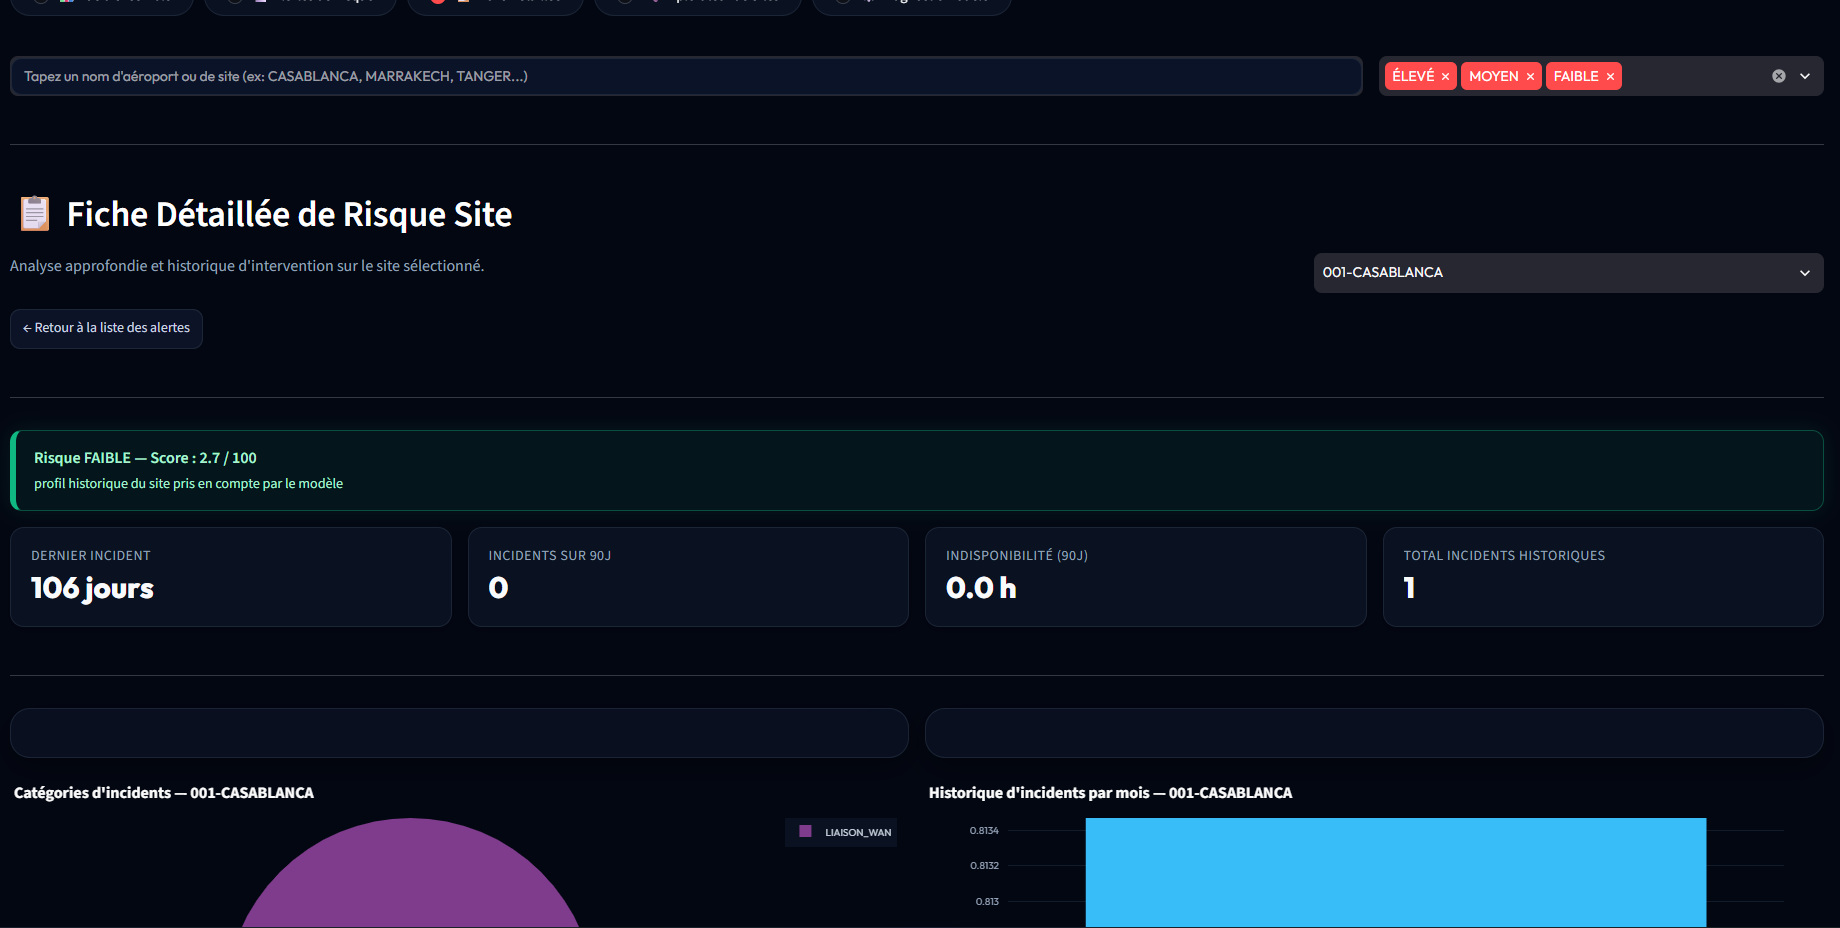
\includegraphics[width=0.95\textwidth,keepaspectratio]{images/onda/onda_detail.png}
\caption[Fiche détaillée d’un site et historique d’incidents.]{Fiche détaillée d’un site et historique d’incidents.}
\end{figure}

\begin{figure}[H]
\centering
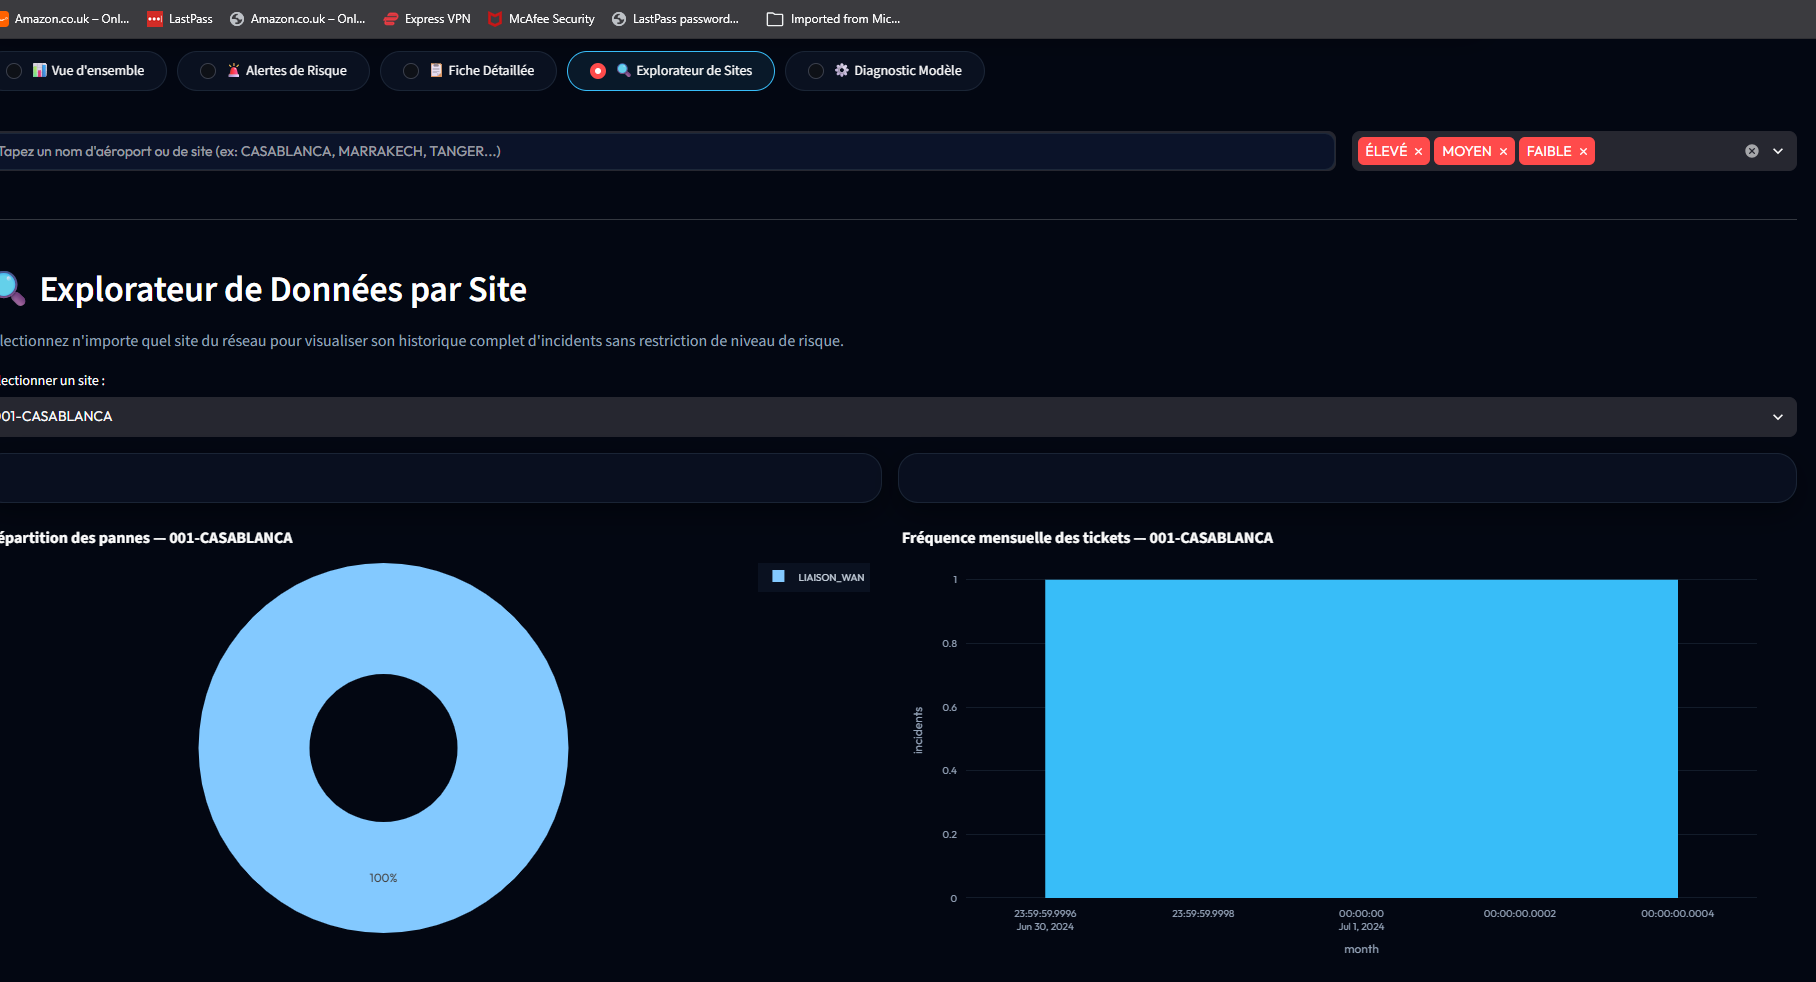
\includegraphics[width=0.95\textwidth,keepaspectratio]{images/onda/onda_explorer.png}
\caption[Explorateur de données par site.]{Explorateur de données par site.}
\end{figure}

À la date de référence, les sites les plus exposés sont 129-OUARZAZATE, 199-ZAGORA, 159-BENS-SLIMANE, 218-BOUARFA et 229-GUELMIM. Par exemple, la fiche de 129-OUARZAZATE affiche un score de 99,9/100, cinq incidents sur 30 jours et 380,8 heures d’indisponibilité sur 90 jours. À l’inverse, la fiche 001-CASABLANCA illustre un site à faible risque avec un score de 2,7/100 et aucune indisponibilité sur 90 jours dans la capture considérée.

La fiche détaillée évite une lecture trop rapide du classement. Elle permet de vérifier si le score est cohérent avec la récence du dernier incident, les événements observés sur 90 jours et la répartition des catégories. L’explorateur apporte une vue complémentaire pour un site qui n’est pas nécessairement dans le top des alertes. L’ingénieur peut ainsi passer du niveau national au diagnostic local sans changer de source de données.

\section{Diagnostic du modèle}

\begin{figure}[H]
\centering
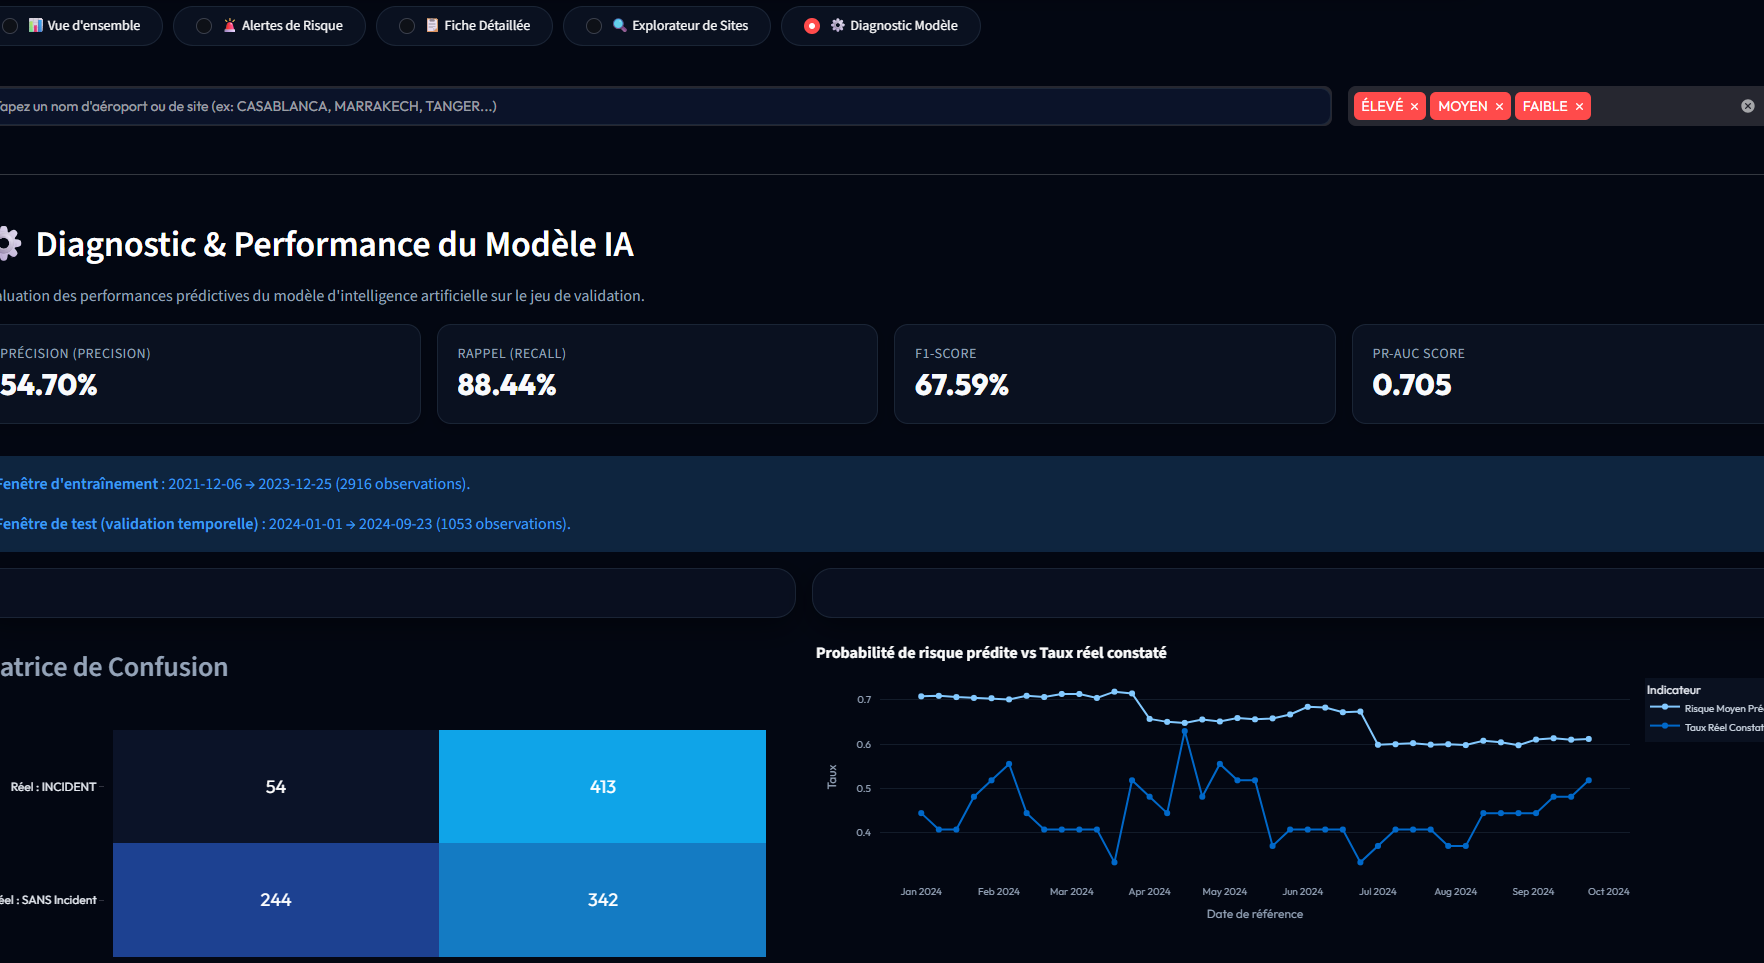
\includegraphics[width=0.95\textwidth,keepaspectratio]{images/onda/onda_model.png}
\caption[Diagnostic du modèle]{Diagnostic du modèle : métriques, matrice de confusion et comparaison temporelle.}
\end{figure}

Le diagnostic rend la performance interprétable par les équipes techniques. La matrice de confusion montre le compromis entre détection et fausses alertes. La courbe de probabilité prédite comparée au taux observé permet de suivre la stabilité du modèle sur la période de test et de repérer les évolutions qui nécessiteraient une réévaluation.

Cette page permet aussi d’installer une culture de suivi du modèle. Une performance mesurée une seule fois ne garantit pas une performance permanente : les habitudes de maintenance, les opérateurs, la topologie et la qualité de saisie peuvent évoluer. Le diagnostic doit donc être consulté lors des réentraînements et après une modification importante du périmètre des sites.

\section{Facteur humain et REX}

\begin{figure}[H]
\centering
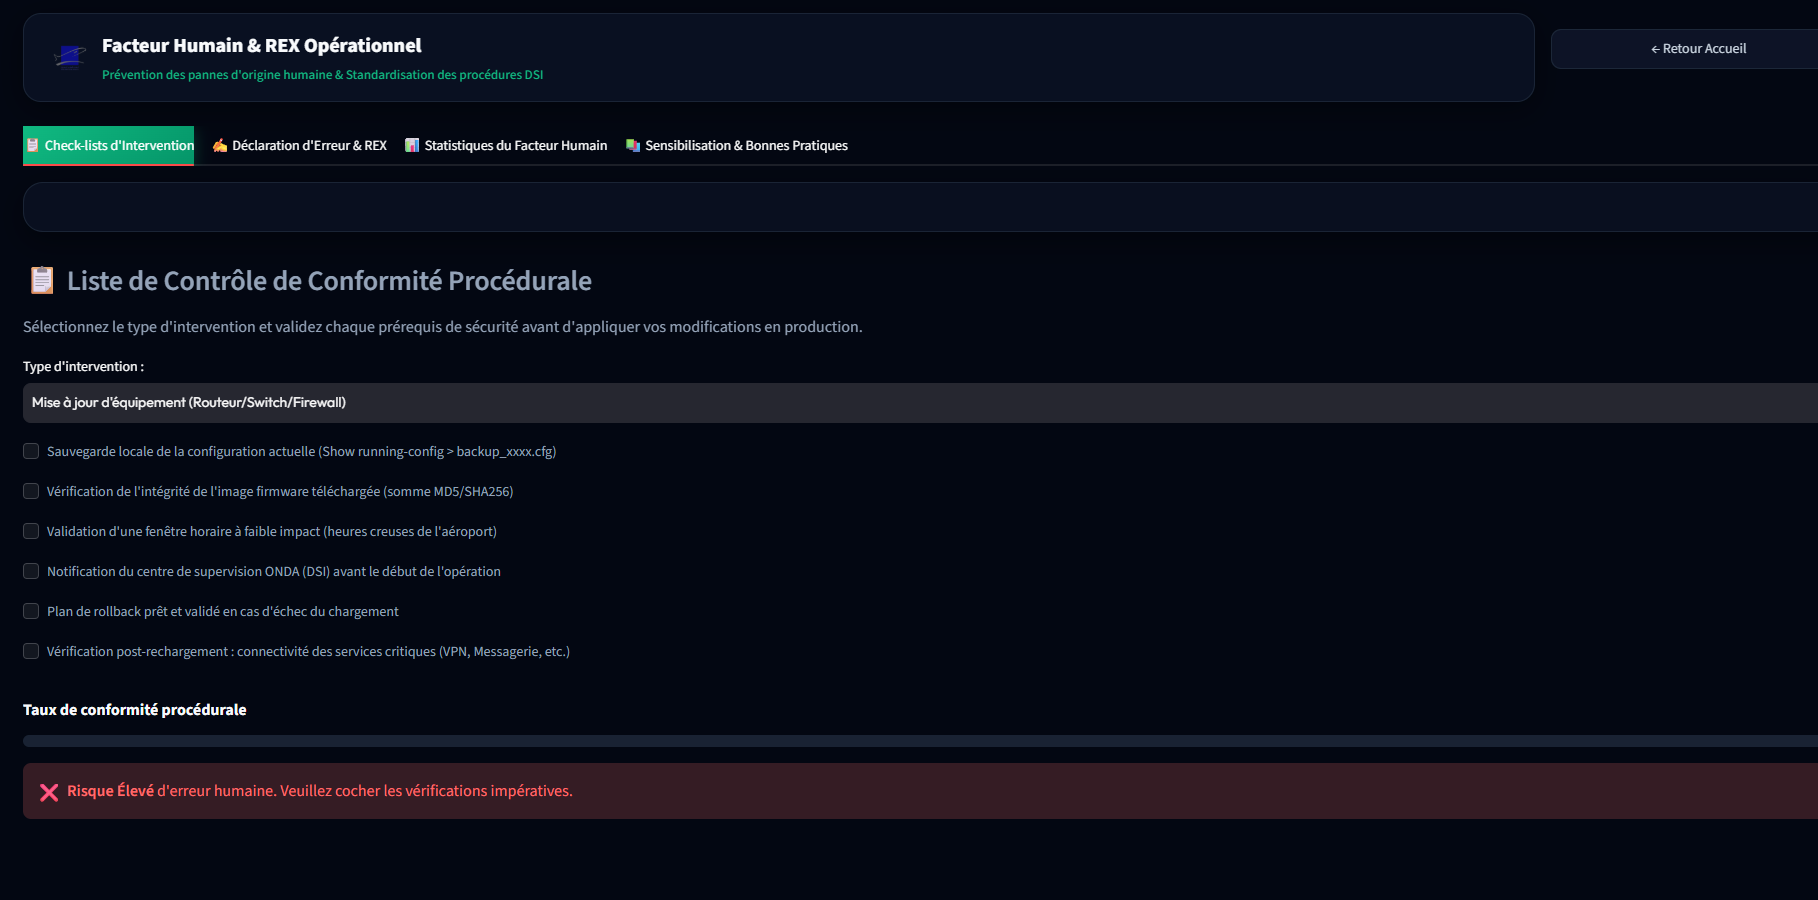
\includegraphics[width=0.95\textwidth,keepaspectratio]{images/onda/onda_human.png}
\caption[Checklist de conformité avant une intervention sur équipement.]{Checklist de conformité avant une intervention sur équipement.}
\end{figure}

Le module impose une vérification avant modification en production : sauvegarde de la configuration, intégrité du firmware, fenêtre horaire, notification du centre de supervision, plan de rollback et contrôle de connectivité après rechargement. Le taux de conformité et l’alerte de risque humain rendent visibles les prérequis non validés. Le REX complète cette approche en conservant les erreurs, leurs causes et les règles à appliquer lors de futures interventions.

L’intérêt de cette checklist est de rendre explicites des gestes parfois considérés comme évidents. Dans une situation urgente, un technicien peut se concentrer sur le rétablissement et oublier la sauvegarde, la notification ou le retour arrière. La plateforme transforme ces points en une étape formelle, mesurable et partageable. Elle ne remplace pas une procédure approuvée, mais elle aide à vérifier que la procédure est appliquée.

\section{Prévention des coupures WAN}

\begin{figure}[H]
\centering
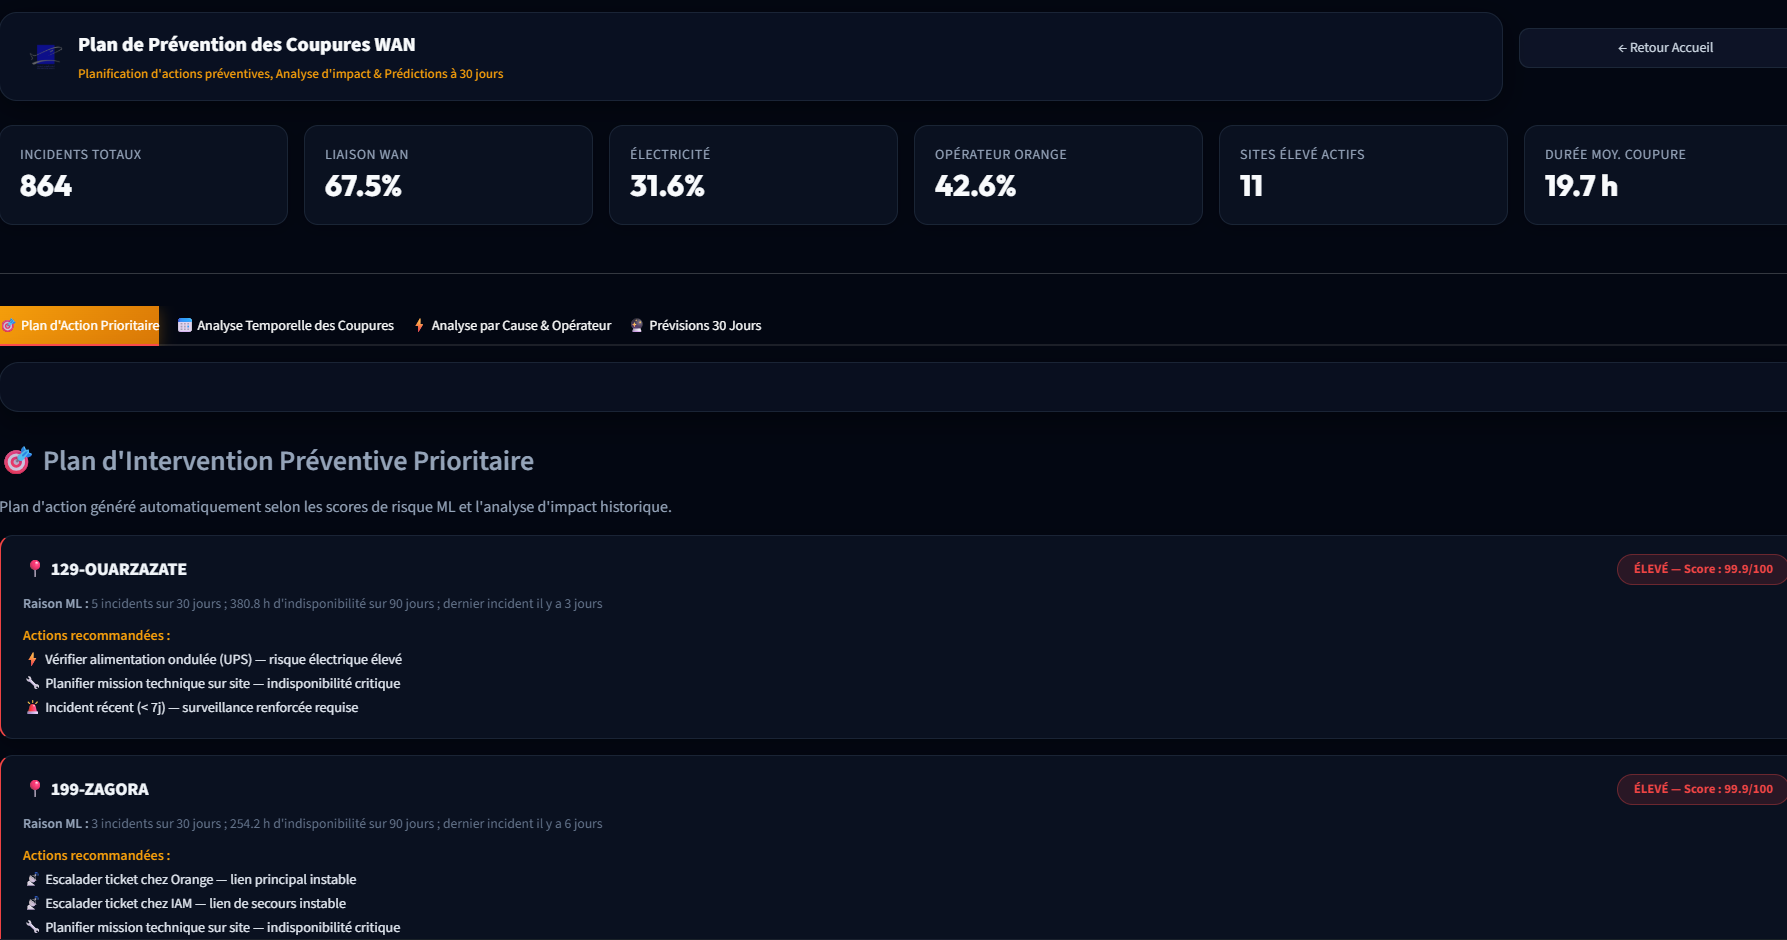
\includegraphics[width=0.95\textwidth,keepaspectratio]{images/onda/onda_prevention.png}
\caption[Plan d’intervention préventive prioritaire.]{Plan d’intervention préventive prioritaire.}
\end{figure}

Le module de prévention agrège les causes et opérateurs associés aux incidents. Il met en évidence la part de la catégorie liaison WAN, la part liée à l’électricité, la contribution d’Orange et le nombre de sites actuellement élevés. Pour chaque site, les recommandations sont formulées en langage opérationnel : vérification de l’UPS, mission technique sur site, surveillance renforcée ou escalade vers l’opérateur concerné.

L’analyse temporelle complète cette lecture en recherchant des périodes où les coupures sont plus fréquentes. Elle peut orienter la planification des contrôles, mais elle doit être interprétée avec le calendrier des travaux, les changements de fournisseur et les événements exceptionnels. Une saisonnalité n’est pas une cause en elle-même ; elle constitue un signal à confronter aux informations de terrain.

\section{Mise en œuvre du CyberRange}

La validation sécurité a été conduite dans un laboratoire Host-Only avec Kali Linux 2024 comme machine d’analyse et Metasploitable 2 comme machine vulnérable. Les captures fournies montrent les adresses 192.168.243.129 pour Kali et 192.168.243.128 pour la cible. Ces adresses sont propres au réseau de laboratoire observé ; elles ne constituent pas une consigne de connexion à une infrastructure réelle.

Le scénario suit une progression pédagogique : identifier les hôtes du laboratoire, observer les services, examiner les traces produites, analyser un artefact et tester des contrôles de détection. La cible est une machine volontairement vulnérable conçue pour l’entraînement. Toutes les manipulations sont réalisées dans le réseau isolé, avec l’objectif de comprendre les preuves et les mesures de défense, et non de reproduire ces actions sur un système tiers.

\begin{figure}[H]
\centering
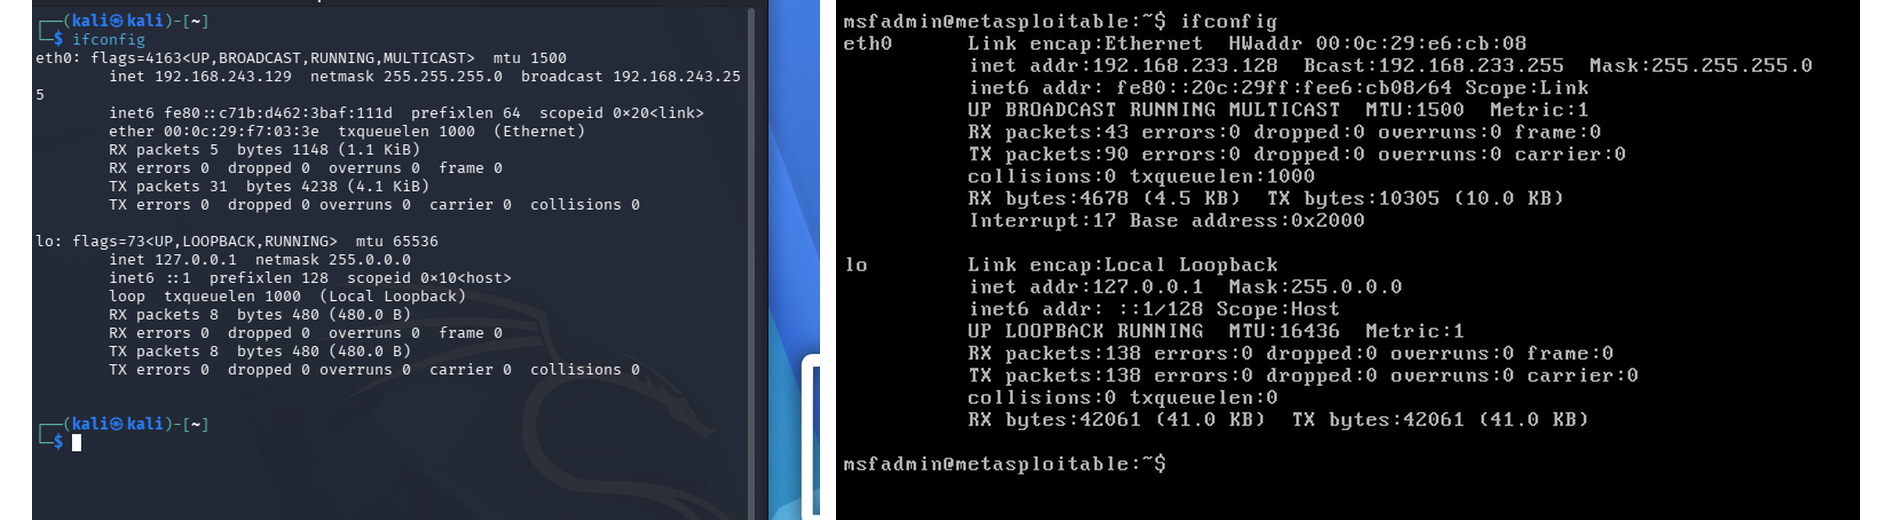
\includegraphics[width=0.95\textwidth,keepaspectratio]{images/cyberrange/cr_network.png}
\caption[Topologie du laboratoire CyberRange isolé.]{Topologie du laboratoire CyberRange isolé.}
\end{figure}

\begin{figure}[H]
\centering
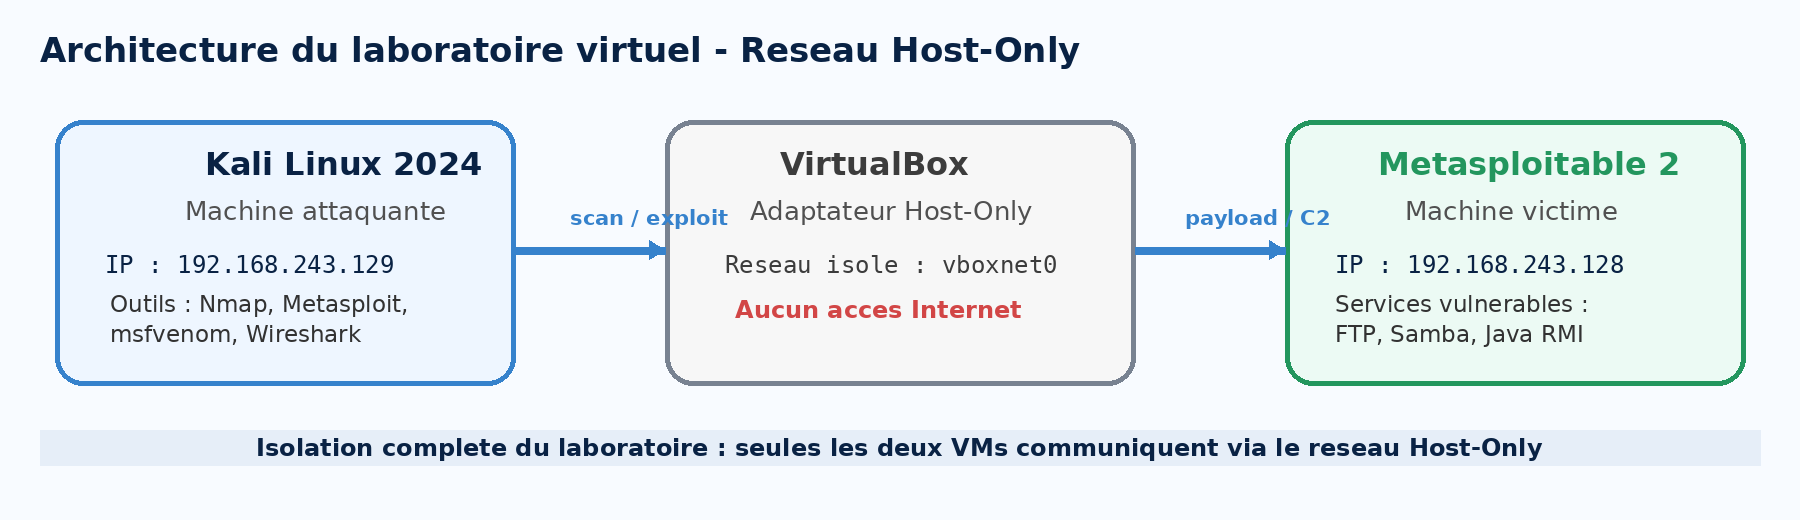
\includegraphics[width=0.95\textwidth,keepaspectratio]{images/cyberrange/cr_architecture.png}
\caption[Architecture pédagogique du CyberRange.]{Architecture pédagogique du CyberRange.}
\end{figure}

\begin{figure}[H]
\centering
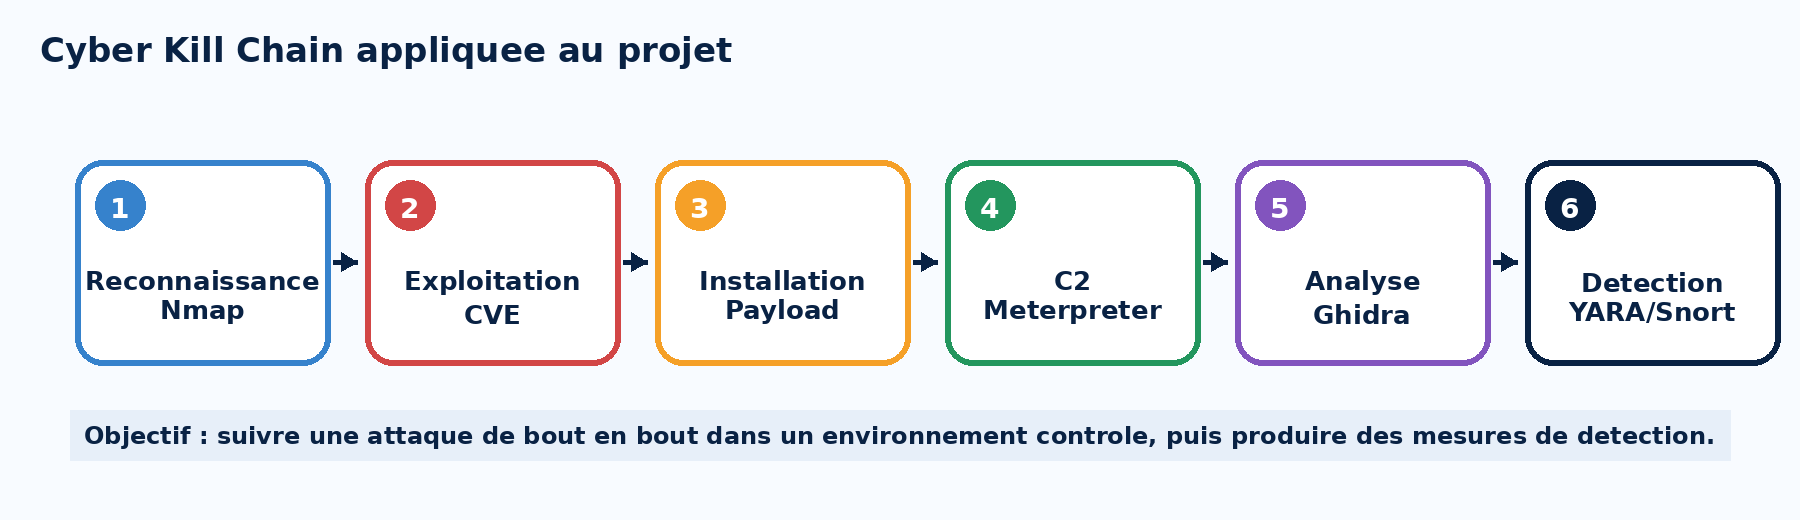
\includegraphics[width=0.95\textwidth,keepaspectratio]{images/cyberrange/cr_killchain.png}
\caption[Déroulement contrôlé du scénario et points de détection.]{Déroulement contrôlé du scénario et points de détection.}
\end{figure}

\subsection{Observation et collecte de preuves}

\begin{figure}[H]
\centering
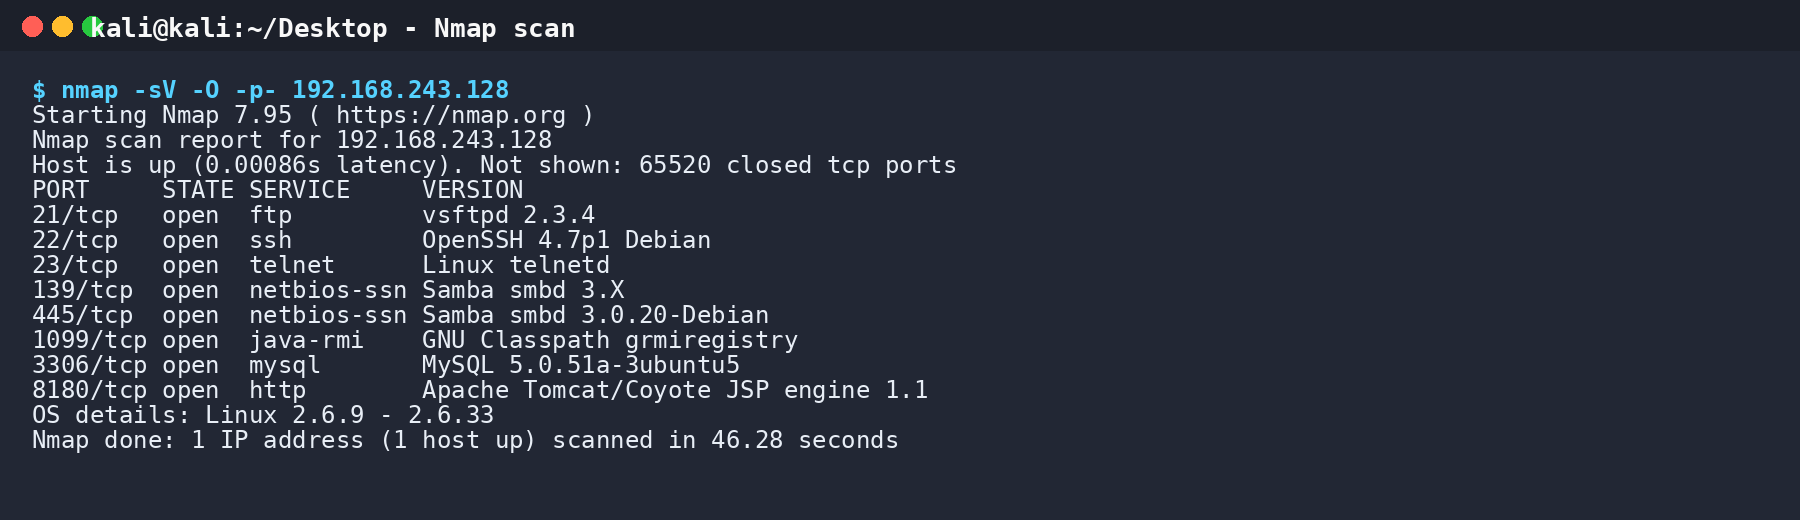
\includegraphics[width=0.95\textwidth,keepaspectratio]{images/cyberrange/cr_nmap.png}
\caption[Observation des services exposés dans le réseau de laboratoire.]{Observation des services exposés dans le réseau de laboratoire.}
\end{figure}

\begin{figure}[H]
\centering
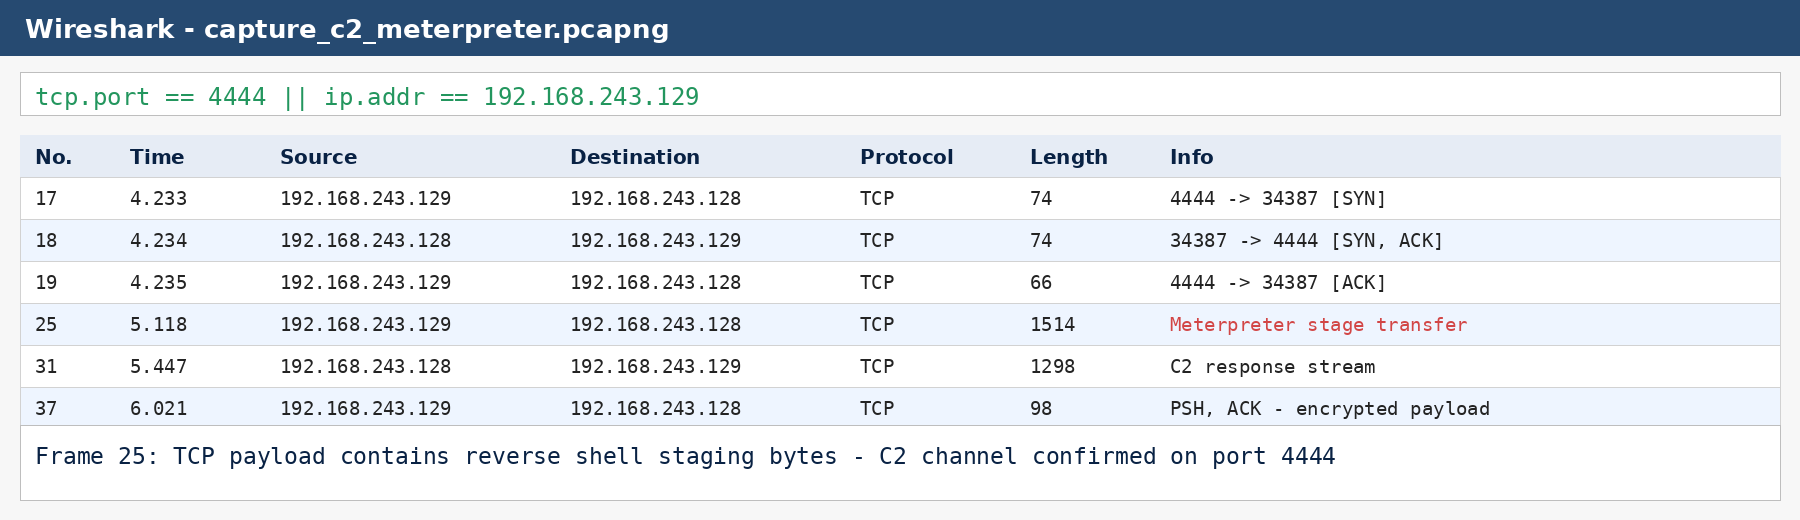
\includegraphics[width=0.95\textwidth,keepaspectratio]{images/cyberrange/cr_wireshark.png}
\caption[Observation des échanges réseau dans Wireshark.]{Observation des échanges réseau dans Wireshark.}
\end{figure}

\begin{figure}[H]
\centering
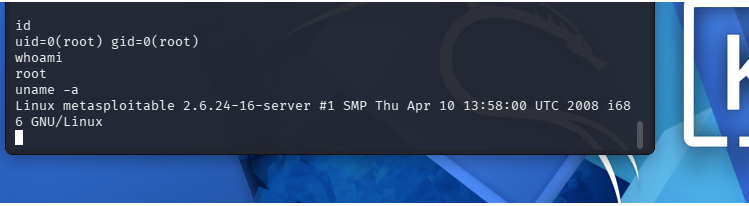
\includegraphics[width=0.95\textwidth,keepaspectratio]{images/cyberrange/cr_shell.png}
\caption[Preuve de session dans l’environnement de test.]{Preuve de session dans l’environnement de test.}
\end{figure}

L’objectif de cette étape est de documenter les traces observables : hôtes, services, échanges, événements et contexte temporel. Les détails d’exploitation ne sont pas reproduits comme une procédure opérationnelle ; le rapport se concentre sur les contrôles, les preuves et la défense.

Les captures réseau permettent de compléter les journaux applicatifs. Elles peuvent révéler une séquence de connexions, un transfert inhabituel ou une communication persistante. Pour être utiles, elles doivent être accompagnées de métadonnées : date, machine utilisée, adresse du laboratoire, filtre appliqué et interprétation. Sans ce contexte, une image isolée est difficile à reproduire et à comparer.

\subsection{Analyse et détection}

\begin{figure}[H]
\centering

\includegraphics[width=0.95\textwidth,keepaspectratio]{images/cyberrange/cr_decompile.png}
\caption[Analyse statique d’un artefact dans Ghidra.]{Analyse statique d’un artefact dans Ghidra.}
\end{figure}

\begin{figure}[H]
\centering
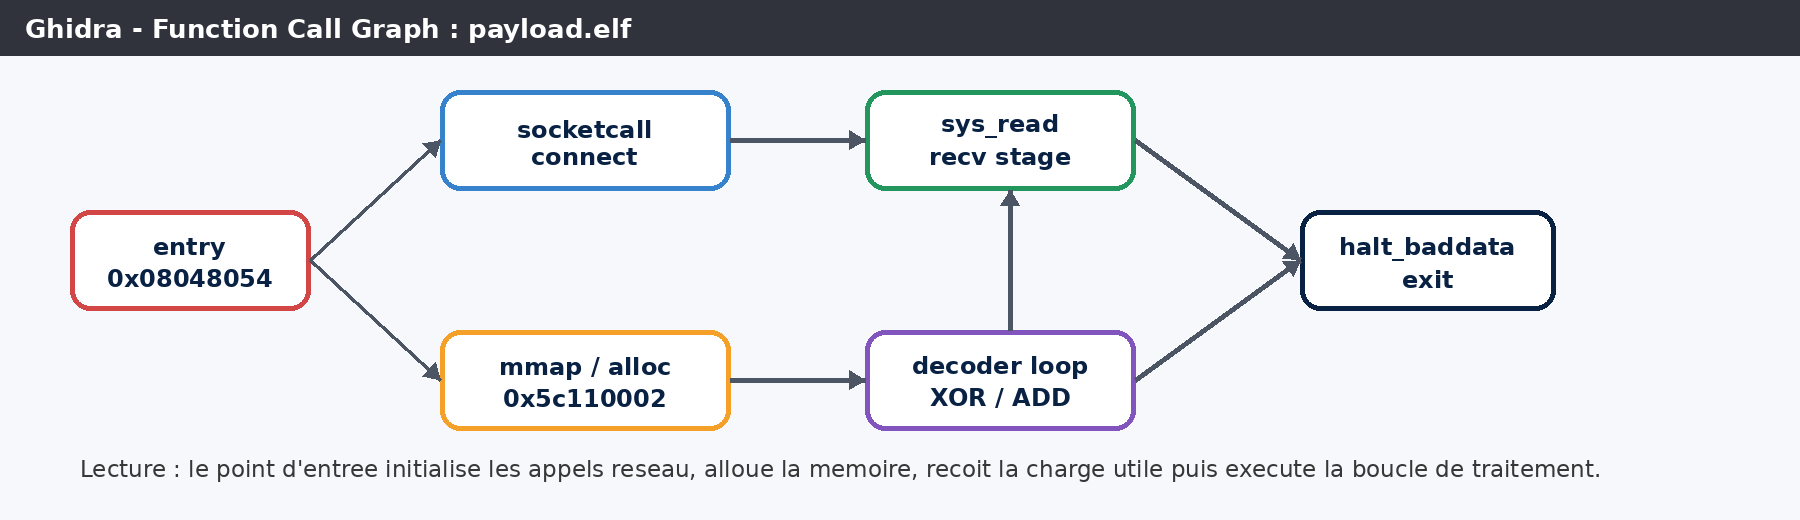
\includegraphics[width=0.95\textwidth,keepaspectratio]{images/cyberrange/cr_ghidra_graph.png}
\caption[Graphe de flux utilisé pour comprendre le comportement de l’artefact.]{Graphe de flux utilisé pour comprendre le comportement de l’artefact.}
\end{figure}

\begin{figure}[H]
\centering

\includegraphics[width=0.95\textwidth,keepaspectratio]{images/cyberrange/cr_yara.png}
\caption[Règle YARA de détection dans le contexte de laboratoire.]{Règle YARA de détection dans le contexte de laboratoire.}
\end{figure}

\begin{figure}[H]
\centering
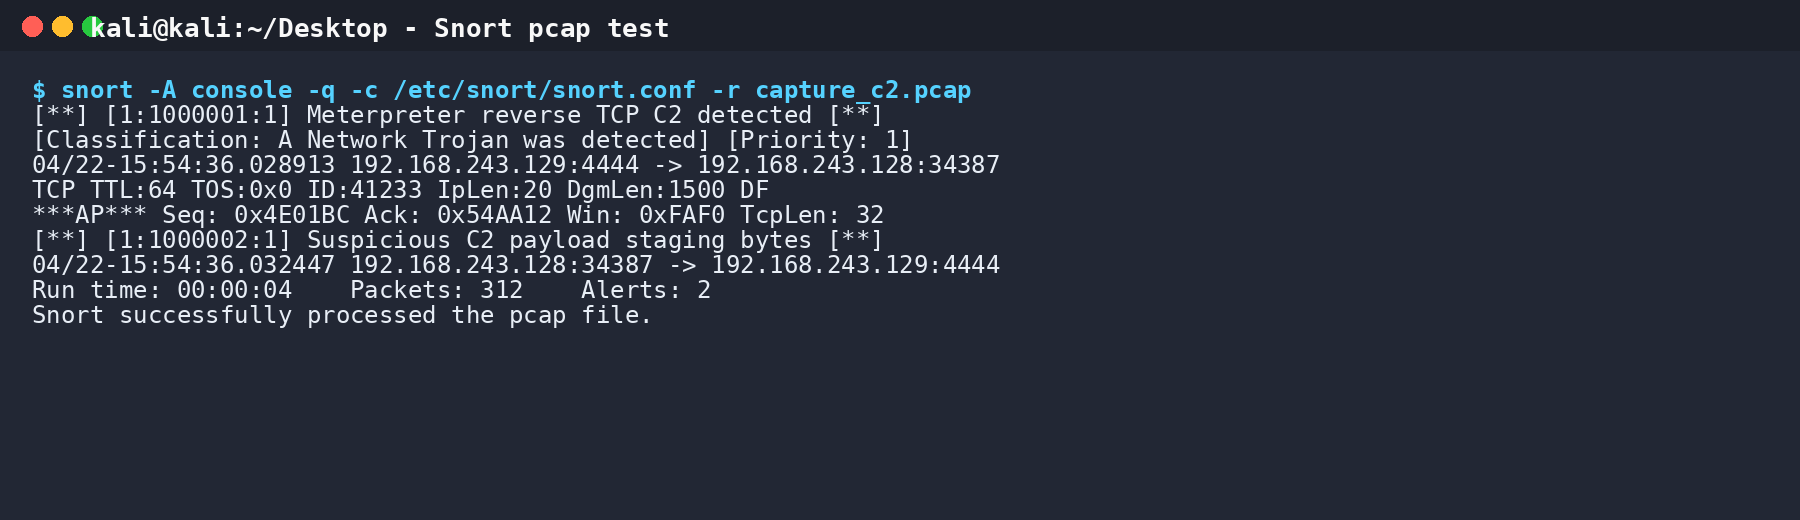
\includegraphics[width=0.95\textwidth,keepaspectratio]{images/cyberrange/cr_snort.png}
\caption[Règle Snort destinée à signaler un indicateur réseau.]{Règle Snort destinée à signaler un indicateur réseau.}
\end{figure}

L’analyse statique et les signatures transforment les observations en contrôles réutilisables. Les règles sont testées uniquement sur les artefacts et flux du CyberRange. Leur transfert vers un environnement ONDA nécessiterait une validation, une adaptation aux journaux disponibles et l’accord des responsables de sécurité.

L’analyse statique aide à repérer des fonctions, des chaînes ou des comportements qui peuvent devenir des indicateurs. Les signatures YARA ciblent des caractéristiques d’un fichier, tandis qu’une règle réseau de type Snort cherche un motif dans un flux. Ces approches sont complémentaires, mais elles peuvent produire des faux positifs et doivent être testées sur des données représentatives avant toute mise en production.

\subsection{Remédiation et REX}

\begin{figure}[H]
\centering
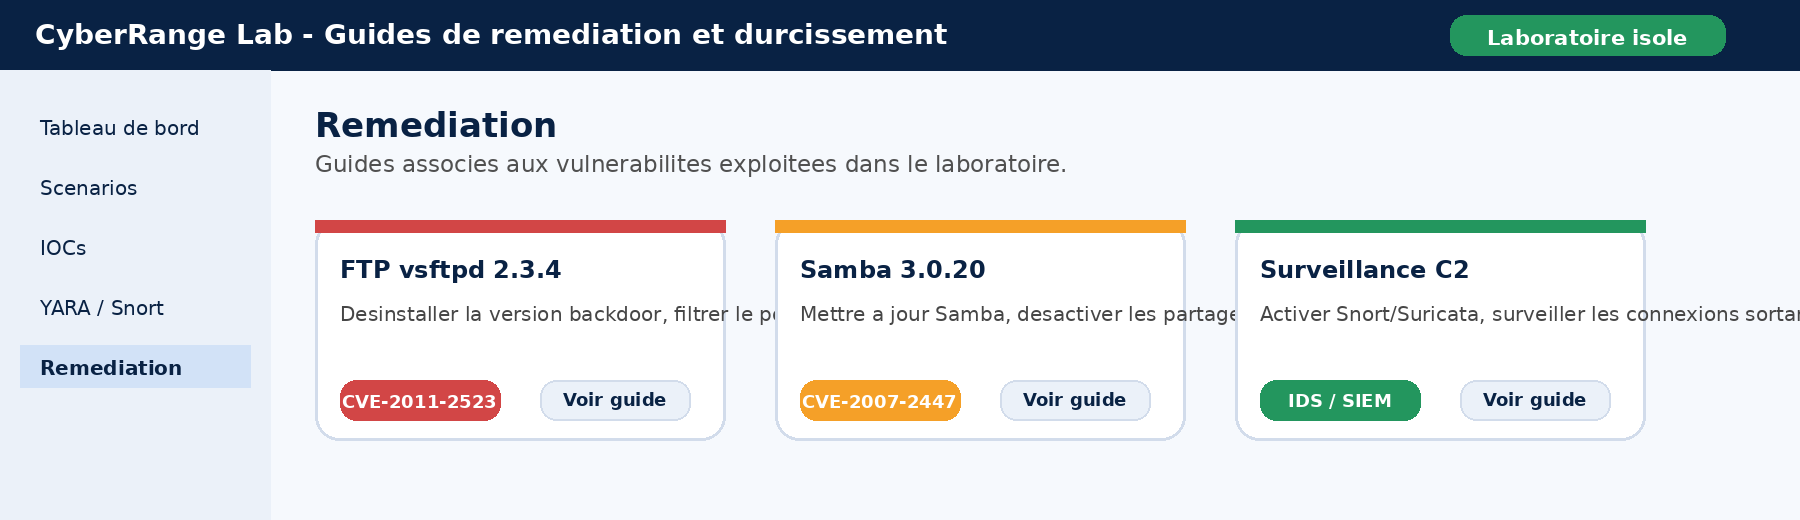
\includegraphics[width=0.95\textwidth,keepaspectratio]{images/cyberrange/cr_remediation.png}
\caption[Mesures de remédiation et de durcissement proposées.]{Mesures de remédiation et de durcissement proposées.}
\end{figure}

\begin{figure}[H]
\centering
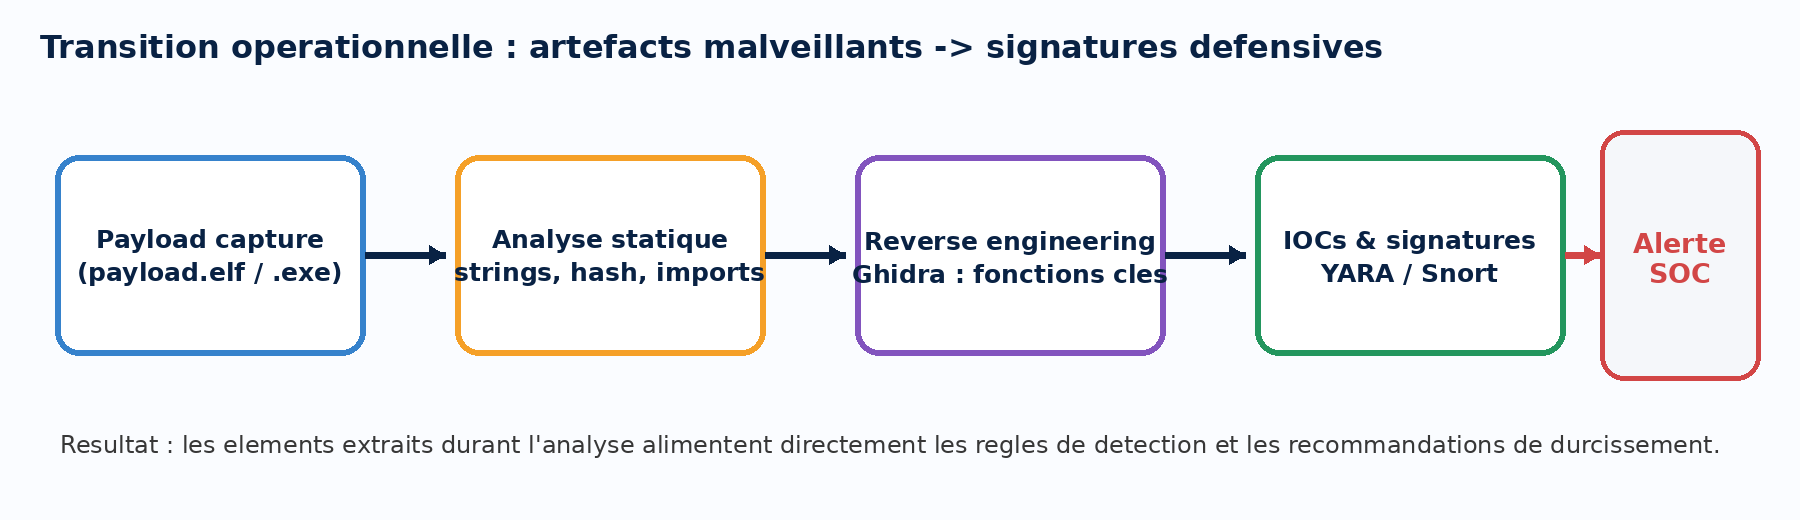
\includegraphics[width=0.95\textwidth,keepaspectratio]{images/cyberrange/cr_transition.png}
\caption[Passage de la preuve technique à la décision défensive.]{Passage de la preuve technique à la décision défensive.}
\end{figure}

La remédiation porte sur la segmentation, la réduction de l’exposition des services, le filtrage, la supervision, la sauvegarde des configurations et la mise à jour maîtrisée. Chaque mesure doit être associée à un responsable, une échéance et une preuve de vérification. Cette logique rejoint le module REX : le résultat de la simulation devient une leçon exploitable dans les futures opérations.

Le passage de la preuve à l’action est essentiel. Une alerte sans responsable peut être ignorée, et une recommandation sans preuve de clôture ne permet pas de vérifier son efficacité. Le REX doit donc décrire le contexte, ce qui a été observé, la décision prise, le résultat obtenu et l’amélioration proposée. Cette structure rend l’expérience utile à une équipe qui n’a pas participé à la simulation initiale.

\section{Limites et précautions}

Les limites concernent à la fois les données, le modèle, l’interface et la simulation. Les résultats présentés sont ceux d’un prototype démontrable à partir des informations disponibles. Une industrialisation demanderait une gouvernance des données, une gestion des accès, un raccordement aux sources opérationnelles et une validation par les responsables de la DSI et de la sécurité.

\begin{itemize}
  \item Les données disponibles permettent principalement un score au niveau du site ; une prédiction au niveau de chaque équipement nécessiterait un identifiant et des attributs d’actif fiables.
  \item Les performances mesurées dépendent de la qualité des tickets, de l’équilibre des classes et de la stabilité des causes déclarées.
  \item Un score élevé signale une priorité de vérification, mais ne prouve pas qu’une coupure aura lieu.
  \item Le CyberRange est un environnement pédagogique isolé ; ses résultats ne doivent pas être généralisés sans validation sécurité et opérationnelle.
  \item Certaines captures de simulation proviennent de scénarios distincts ; elles sont présentées comme preuves complémentaires et non comme une session unique non documentée.
\end{itemize}

\section{Conclusion}

La réalisation met en œuvre une plateforme capable de passer de l’historique de maintenance à une décision priorisée. Les interfaces couvrent la vision exécutive, le diagnostic technique, la checklist humaine et la prévention WAN. La validation CyberRange ajoute une dimension de détection et de remédiation, tout en conservant l’isolement nécessaire. L’ensemble constitue une base cohérente pour améliorer progressivement la qualité des données, la précision du modèle et l’intégration aux processus réels de la DSI.

La valeur principale du système est donc la continuité du parcours : comprendre le risque, décider d’une vérification, contrôler l’intervention, observer les résultats et mémoriser l’expérience. Cette continuité donne une cohérence aux différents modules et permet d’envisager des améliorations futures sans perdre l’objectif initial de prévention des interruptions.


\frontchapter{Conclusion générale}
Ce projet a permis de concevoir une approche intégrée de l’analyse des risques et des alertes prédictives à partir des données de maintenance des actifs informatiques de l’ONDA. En exploitant les historiques de 27 sites WAN, la plateforme calcule un score à 30 jours, classe les priorités et propose des actions de prévention compréhensibles par les équipes. Le portail exécutif facilite la décision, le module de risque rend les indicateurs et les performances du modèle visibles, le module facteur humain réduit les oublis avant intervention et le REX organise la capitalisation. Chaque composant répond ainsi à une étape du même problème : éviter qu’un signal connu ne soit ignoré jusqu’à devenir une interruption coûteuse.

La simulation menée dans un CyberRange Host-Only complète cette vision en donnant un cadre contrôlé pour observer des traces, tester des détections et formaliser des mesures de remédiation. Elle rappelle que la disponibilité d’un service ne dépend pas uniquement d’un équipement ou d’un opérateur ; elle dépend aussi de la capacité à surveiller, à réagir et à apprendre. Les preuves techniques obtenues dans le laboratoire peuvent donc servir de support pédagogique pour discuter la segmentation, le filtrage, la supervision et la documentation des incidents.

Les résultats doivent toutefois être interprétés avec prudence. Le modèle décrit principalement un risque au niveau site, dépend de la qualité des tickets et reste une aide à la décision. La performance mesurée doit être suivie dans le temps, les faux positifs doivent être analysés et toute alerte doit être confrontée au contexte opérationnel. De la même manière, les règles de détection issues du CyberRange ne peuvent pas être appliquées directement à la production sans validation, adaptation et accord des responsables compétents.

Les perspectives sont l’enrichissement du référentiel d’actifs, l’ajout de données de topologie et de supervision temps réel, le suivi du drift du modèle, l’intégration d’une authentification et d’un journal d’audit, ainsi que la validation progressive des règles de détection dans un environnement conforme aux procédures de sécurité de l’ONDA. À terme, cette évolution pourrait fournir un historique complet reliant l’état d’un site, son risque estimé, les interventions réalisées, les preuves observées et l’efficacité des mesures prises.

\clearpage
\frontchapter{Bibliographie et Nétographie}
\begin{enumerate}[label={[\arabic*]},leftmargin=1.0cm]
\item Documentation Python, Python Software Foundation, \url{https://docs.python.org/3/}.
\item Scikit-learn, \emph{User Guide -- Logistic Regression and model evaluation}, \url{https://scikit-learn.org/stable/user_guide.html}.
\item Pandas Documentation, User Guide, \url{https://pandas.pydata.org/docs/}.
\item VirtualBox User Manual, Oracle, \url{https://www.virtualbox.org/manual/}.
\item Wireshark Documentation, User's Guide, \url{https://www.wireshark.org/docs/}.
\item Ghidra Documentation, National Security Agency, \url{https://ghidra-sre.org/}.
\item YARA Documentation, \url{https://yara.readthedocs.io/}.
\item Snort Documentation, Cisco Talos, \url{https://www.snort.org/documents}.
\item MITRE ATT\&CK, Enterprise Matrix, \url{https://attack.mitre.org/}.
\item OWASP, Secure Coding Practices and Application Security Verification resources, \url{https://owasp.org/}.
\item Documentation interne du projet ONDA : historiques d’incidents, écrans de la plateforme et résultats d’évaluation, 2024.
\item Rapport technique CyberRange du binôme, éléments de laboratoire et captures intégrées au présent rapport.
\end{enumerate}

\clearpage
\frontchapter{Annexes}
\section*{Annexe A -- Principaux indicateurs du projet}
\begin{table}[H]
\centering
\small
\caption{Récapitulatif des indicateurs.}
\begin{tabularx}{\textwidth}{B{8.5cm} X}
\toprule
Indicateur & Valeur\\
\midrule
Incidents historiques analysés & 864\\
Sites aéroportuaires & 27\\
Horizon de prédiction & 30 jours\\
Accuracy & 62,39\%\\
Précision & 54,70\%\\
Rappel & 88,44\%\\
F1-score & 67,59\%\\
PR-AUC & 0,705\\
\bottomrule
\end{tabularx}
\end{table}

\section*{Annexe B -- Périmètre de la simulation}
La simulation est limitée à un réseau Host-Only contrôlé, à des machines prévues pour la formation et à des objectifs de détection/remédiation. Elle ne fournit aucune autorisation d’essai sur le réseau ONDA ou sur un tiers. Toute reprise opérationnelle doit faire l’objet d’une validation formelle, d’un périmètre défini et d’une supervision compétente.

\end{document}
